% Activate the following line by filling in the right side. If for example the name of the root file is Main.tex, write
% "...root = Main.tex" if the chapter file is in the same directory, and "...root = ../Main.tex" if the chapter is in a subdirectory.
 
% !TEX root = ../thesis.tex 

\chapter[Surface-based PV estimation]{Surface-based partial volume estimation}
\label{tob_pv_chapter}

\section{Introduction}

Although surface-based segmentation is well-established within the literature, the same is not true of surface-based PV estimation\footnote{The majority of the work presented in this chapter has been published as T. Kirk, T. Coalson, M. Craig and M. Chappell, ``Toblerone: surface-based partial volume estimation'', IEEE Transaction on Medical Imaging, vol. 39 no. 5, pp 1501 - 1510, 2020.}. A surface-based approach could bring two key advantages. Firstly, if it is true that surface segmentations of particular structures are more accurate than their volumetric counterparts, then the same could also be true of PV estimates derived from these (although the accuracy of any such estimates will be constrained by that of the surfaces from which they are derived). This would in turn have implications for the efficacy of PVEc within these structures. Secondly, a surface-based approach allows PVs to be obtained in any voxel grid without recourse to resampling. This is beneficial for minimising the mixing of signal that is introduced by resampling, an artefact that cannot be fully accounted for by subsequent correction (as was demonstrated in chapter \ref{pvec_chapter}). 

Conceptually, surface-based PV estimation approaches the problem in a purely geometric manner: \textit{given a patch of surface that intersects a voxel, what is the volume on either side of the surface that is bounded by the voxel?} It is this formulation that makes the approach immune to the problems of resampling. For a given surface intersecting a voxel grid, any transformation can be performed by manipulating the voxel grid (for example, a translation, rotation or scaling) independent of the surface itself. This means that the boundaries of the anatomical structure represented by the surface are conserved. This same is not true of a volumetric approach: in that case, the boundaries of the structure have been reduced to a voxel-wise representation (the result of volumetric segmentation), and therefore any transformation operation must be applied to the voxel representation of the structure, which will in turn entail interpolation across structure boundaries at the cost of edge definition. The consequences of this are illustrated in greater detail in figure \ref{resampling_demo}. 

\begin{figure}
\centering
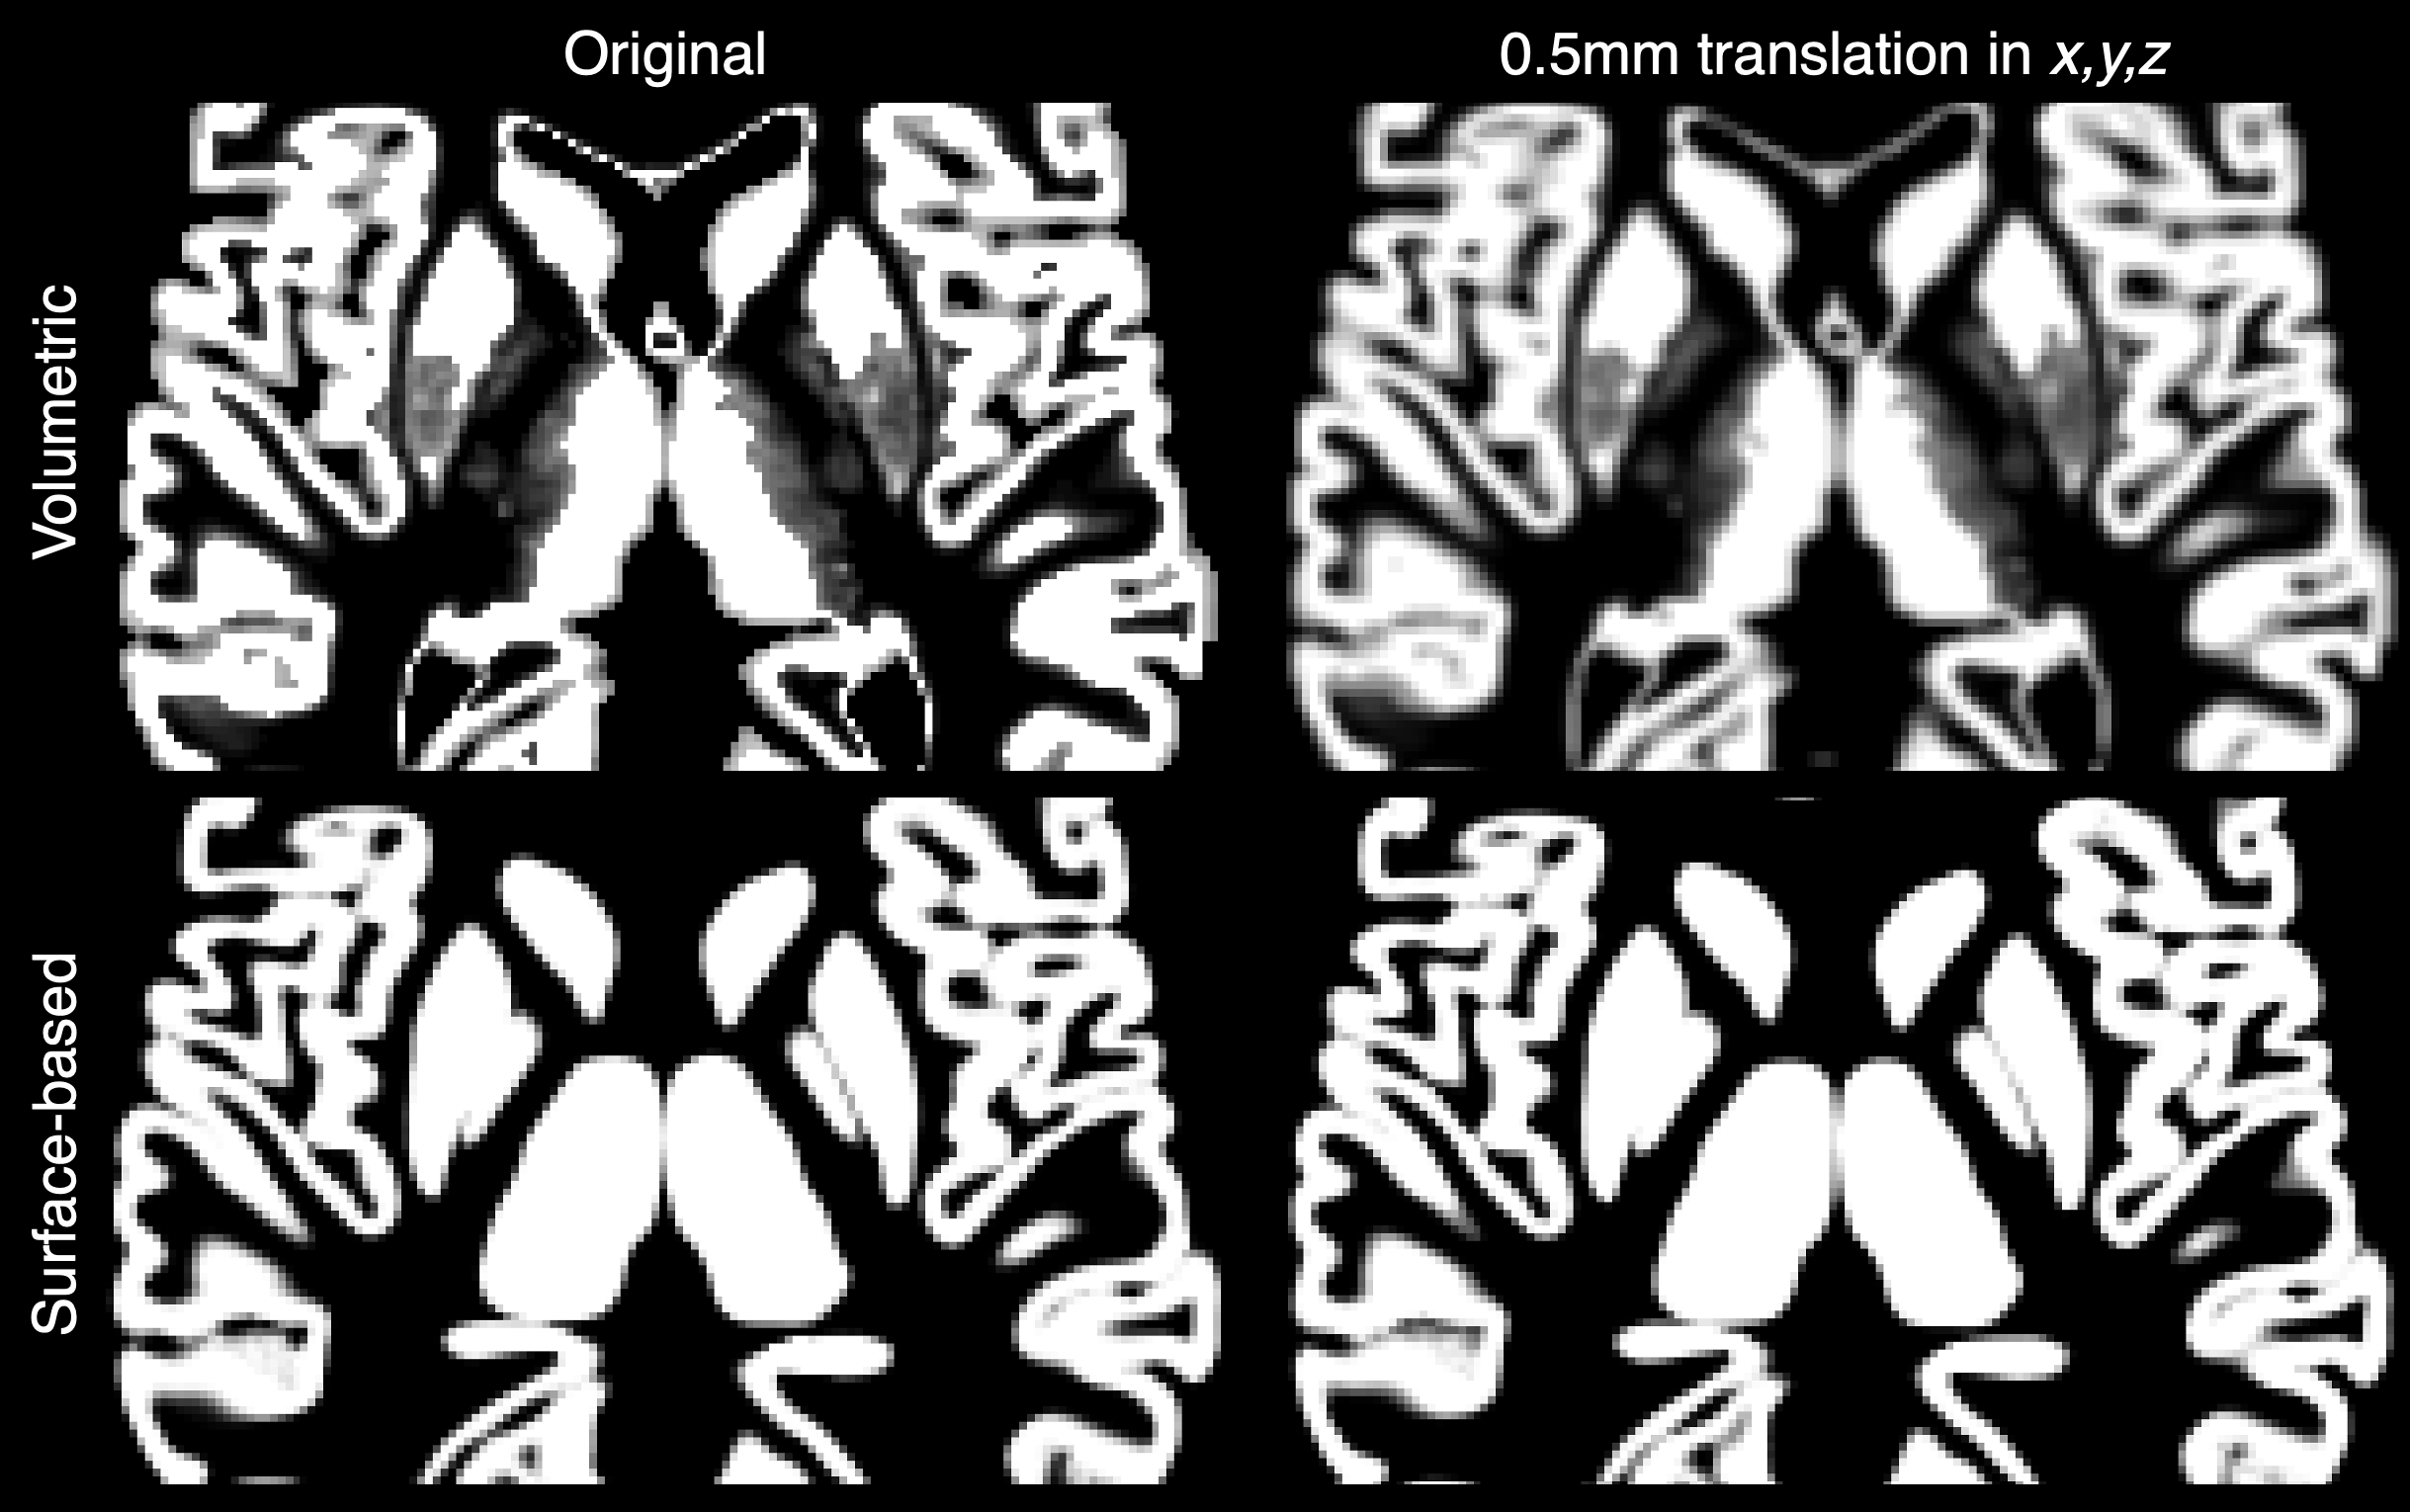
\includegraphics[width = \textwidth]{resampling.png}
\caption{Illustration of resampling-induced blurring on a 1mm isotropic GM PV map. The left column shows the original estimates produced by a volumetric method (FSL FAST) and a surface-based method (Toblerone, the subject of this chapter); the right shows the result of a 0.5mm translation along each axis. For a volumetric method, any transformation will require a resampling operation that blurs the boundaries of underlying structure. For a surface-based method, the same transformation can be achieved by manipulating the voxel grid independently of the surface itself, hence avoiding resampling and the accompanying blurring.}
\label{resampling_demo}
\end{figure}

Although some surface-based PV estimation tools exist in the literature, past efforts have usually been designed with a specific modality in mind. Two notable examples for neuroimaging are the ribbon-constrained (RC) method used within the HCP's \textit{fMRISurface} pipeline \cite{Glasser2013} and PETSurfer \cite{Greve2016, Greve2014}, a variant of FreeSurfer. The former is designed for use with BOLD and so distinguishes only between cortex and otherwise, not the GM, WM and non-brain required by other modalities; whereas the latter is both PET-specific and tightly integrated into FreeSurfer such that it is hard to use independently of that workflow. One of the few examples of a generally applicable method that is not tied to any particular modality is NeuropolyPVE, though that is also constrained to use with the cortex only \cite{NeuropolyPVE}. It should also be noted that FreeSurfer itself, which is widely used to generate the surfaces on which these methods operate, does offer some tools to perform surface-based PV estimation for the cortex only (and not the subcortex). It is however somewhat difficult to use the outputs of these tools independently of the wider FreeSurfer workflow, which means they are awkward to integrate into a general purpose analysis pipeline with PVEc. 

The objective of this work was to develop an algorithm, named Toblerone, to estimate partial volumes for both cortical and subcortical structures (where such surfaces are available, for example via FSL FIRST \cite{Patenaude2011}) for neuroimaging applications. The end result is highly general and could be used with data from multiple modalities and/or in other parts of the body. 

\section{Theoretical foundation}

Voxelisation is the process of quantifying the volume contained within a surface and many algorithmic implementations are given in the computer graphics literature. The key step within this operation is determining if a point lies interior or exterior to a given surface; by repeating this test entire volumes can be built up. The ray intersection test outlined by Nooruddin and Turk is widely used for this and requires only that the surfaces be contiguous (water-tight) \cite{Nooruddin2003}. The test is performed by projecting an infinite ray in any direction from the point under test and counting the number of intersections made with the surface. A ray from an interior point will make an odd number of intersections as it exits the surface (including folds within the surface, there will be one more point of exit than entry); conversely an exterior point will make an even number of intersections (balanced entries and exits), if at all. This test scales badly with increasing spatial resolution: for a linear resolution of $n$ samples per unit distance, $n^3$ tests per unit volume are required. Furthermore, as each ray must be tested against each surface element, the test also becomes more complex for increasing surface resolution (linearly for a naïve implementation). For a typical functional image of 10\textsuperscript{5} voxels and 2.5x10\textsuperscript{5} surface elements in a FreeSurfer cortical surface, this is prohibitively computationally intensive.

The method adopted in this work is to only use the portion of surface that actually intersects a given voxel (termed the \textit{local patch}) for ray intersection testing. The local patch is defined as all triangles that intersect the voxel or, equivalently, the minimal set of triangles that unambiguously divides the voxel into two regions. This patch is by definition non-contiguous, so it is necessary to modify the ray intersection test accordingly; the modified form is referred to as the ‘reduced’ test in contrast to the ‘classical’ test. Within each voxel, a \textit{root point} that is known to lie within the surface is identified via the classical ray test. Any other point within the voxel may then be tested by projecting the finite line segment 

\begin{equation}
\vec{r} = \vec{p_t} + \lambda(\vec{p_r} - \vec{p_t})
\end{equation} 

where $\vec{p_t}$ is the point under test, $\vec{p_r}$ is the root point and $0 \leq \lambda \leq 1$ is a distance multiplier along the line. A parity test is then applied to the number of intersections identified between the root and test points. The fact that the line terminates at a point interior to the surface means that exterior points will lead to one more point of entry than exit; conversely interior points will lead to either zero or an even number of intersections. It is not necessary to test surface elements outside the voxel as the finite length of the line segment means it can never leave the voxel. Figure \ref{raytest} provides an illustration of the test in practice. 

\begin{figure}
\centering
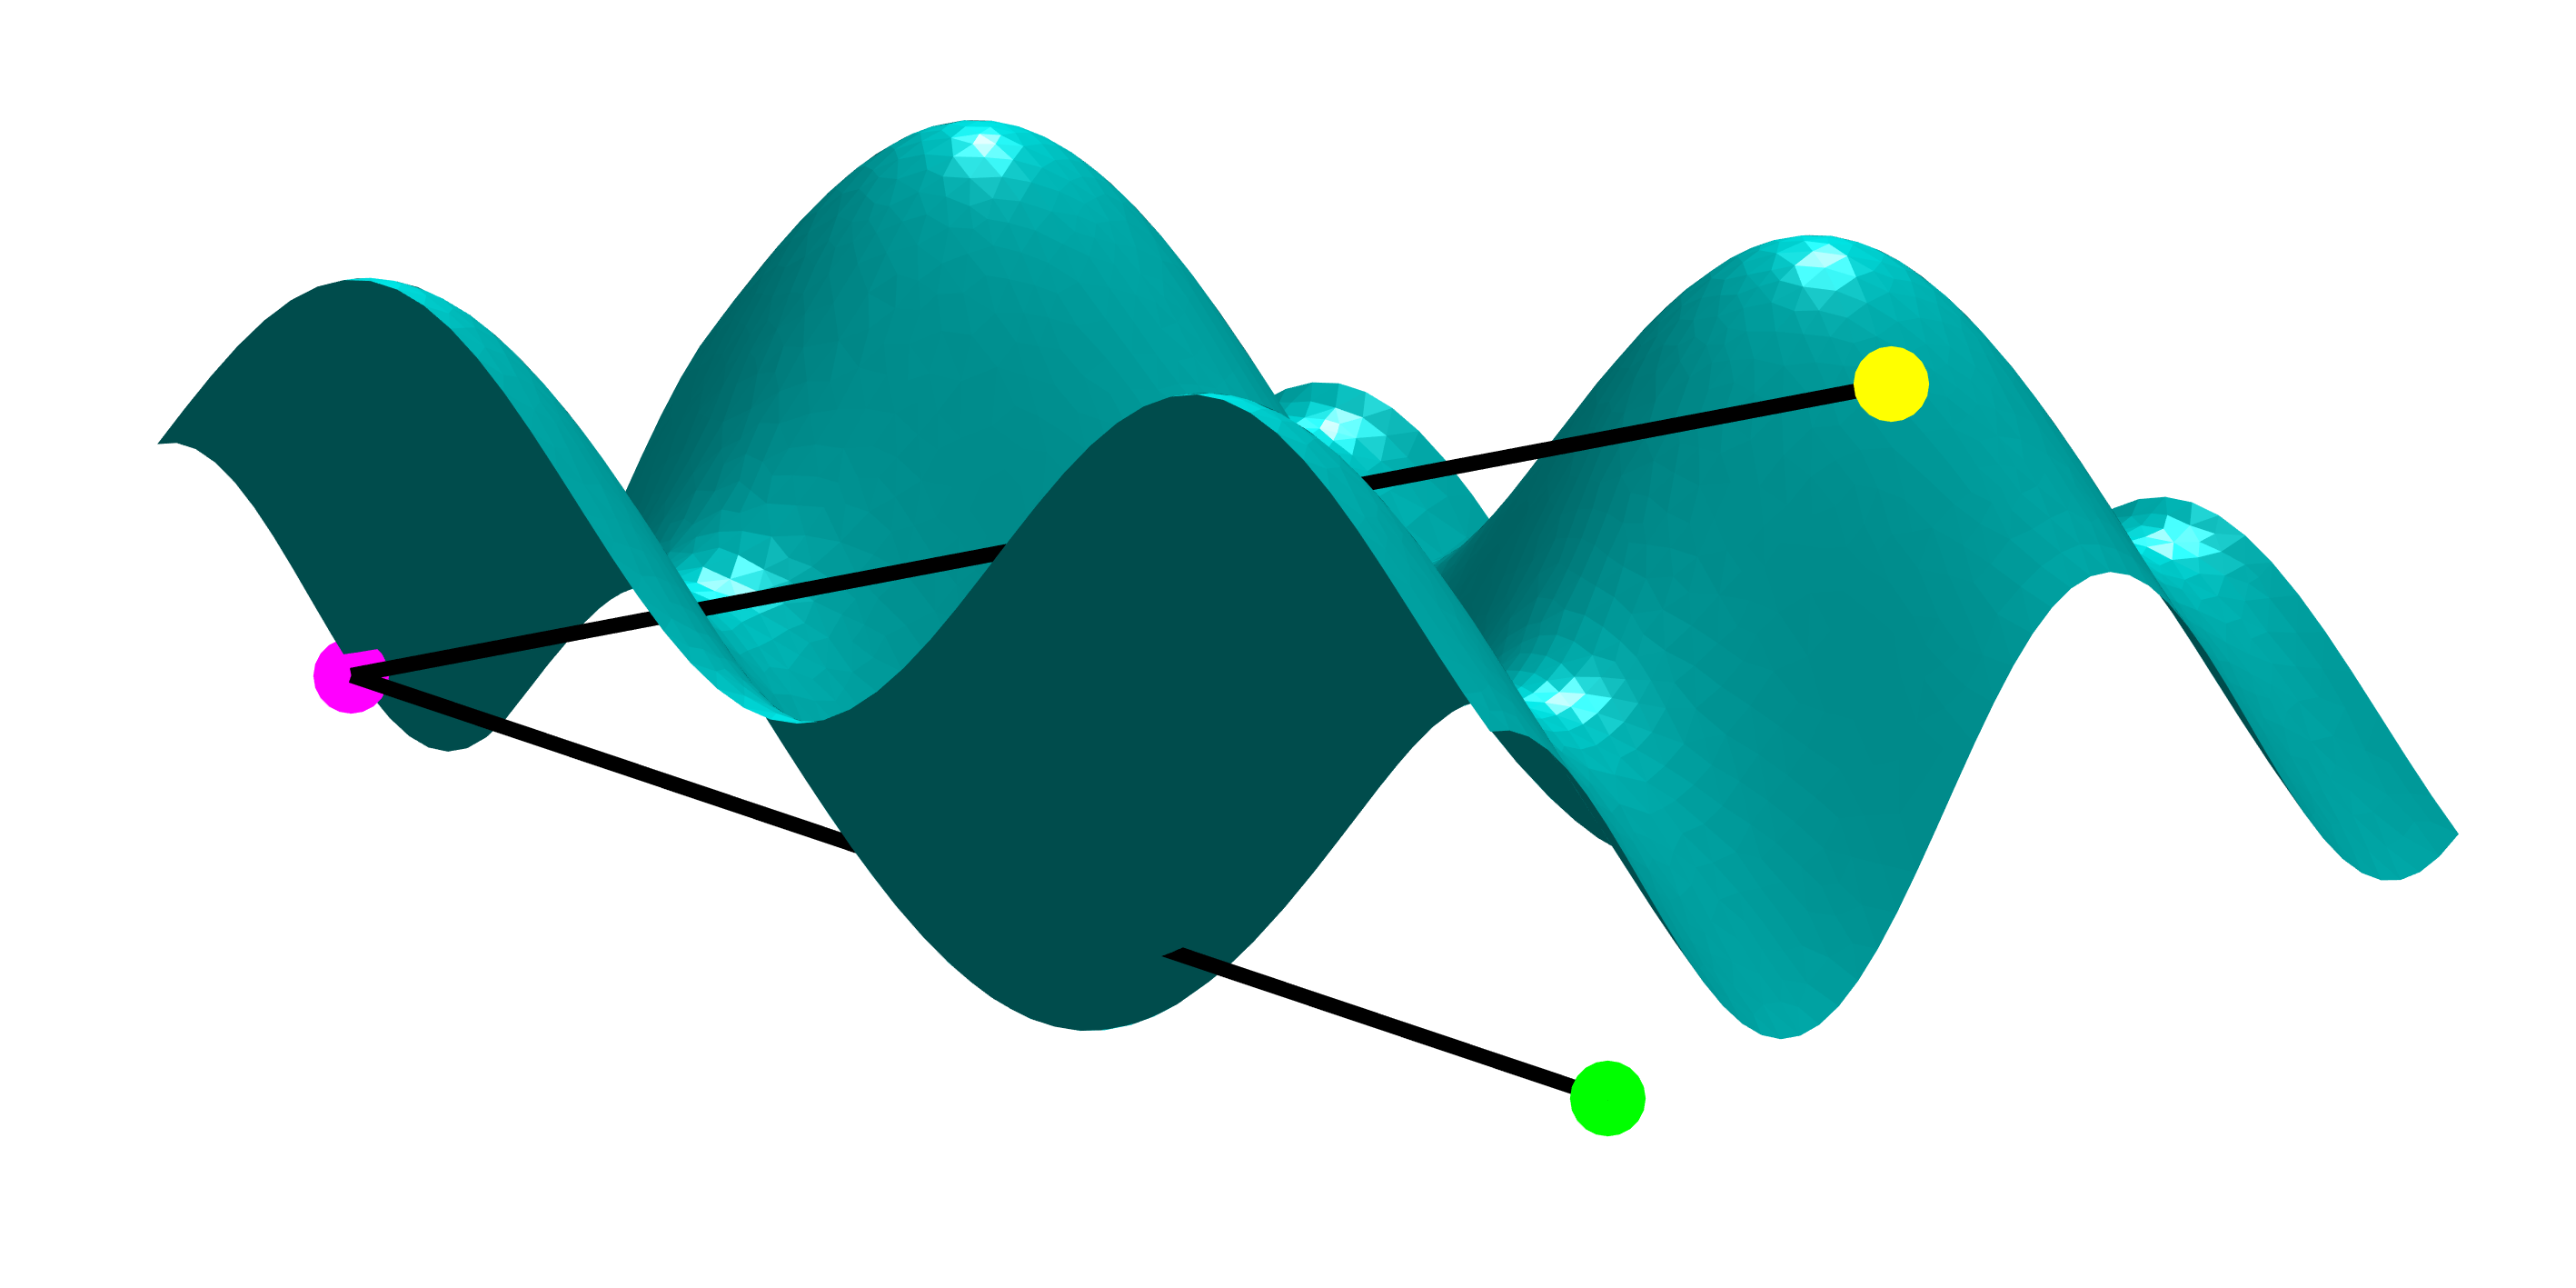
\includegraphics[width = 0.8\textwidth]{raytest.png}
\caption{Reduced ray intersection test for non-contiguous surfaces. The root point (interior) is shown in magenta. A ray from an interior point (green) makes two intersections due to the presence of a fold; from an exterior point (yellow) there is one intersection.}
\label{raytest}
\end{figure}

In order to minimise the number of tests required per voxel, convex hulls (defined as the smallest possible region enclosing a set of points within which any two points can be connected without leaving the region \cite{DeBerg2008}) are used to estimate partial volumes wherever possible. The rationale for this is that if the extrema points of a region can be classified as interior/exterior to a surface then, to an approximation, all points lying within the convex hull of these points will share the same classification. 

\section{Algorithmic implementation}

The following section addresses PV estimation for structures within the brain, for which the tissue classes of interest are GM, WM and non-brain. The same principles would apply to structures in other areas of the body, though the interpretation of tissue classes would differ. 

\subsection{Estimation for a single surface}

The core algorithm within Toblerone estimates the voxel-wise interior/exterior PVs arising from the intersection of a single surface with an arbitrary voxel grid. Toblerone assumes cuboid voxels with a ‘boxcar’ (PSF), which is to say that it does not allow for any mixing of signal between voxels. In reality, different modalities have differing PSFs and such effects may be separately accounted for via a modality-specific convolution operation. 

\begin{figure}
\centering
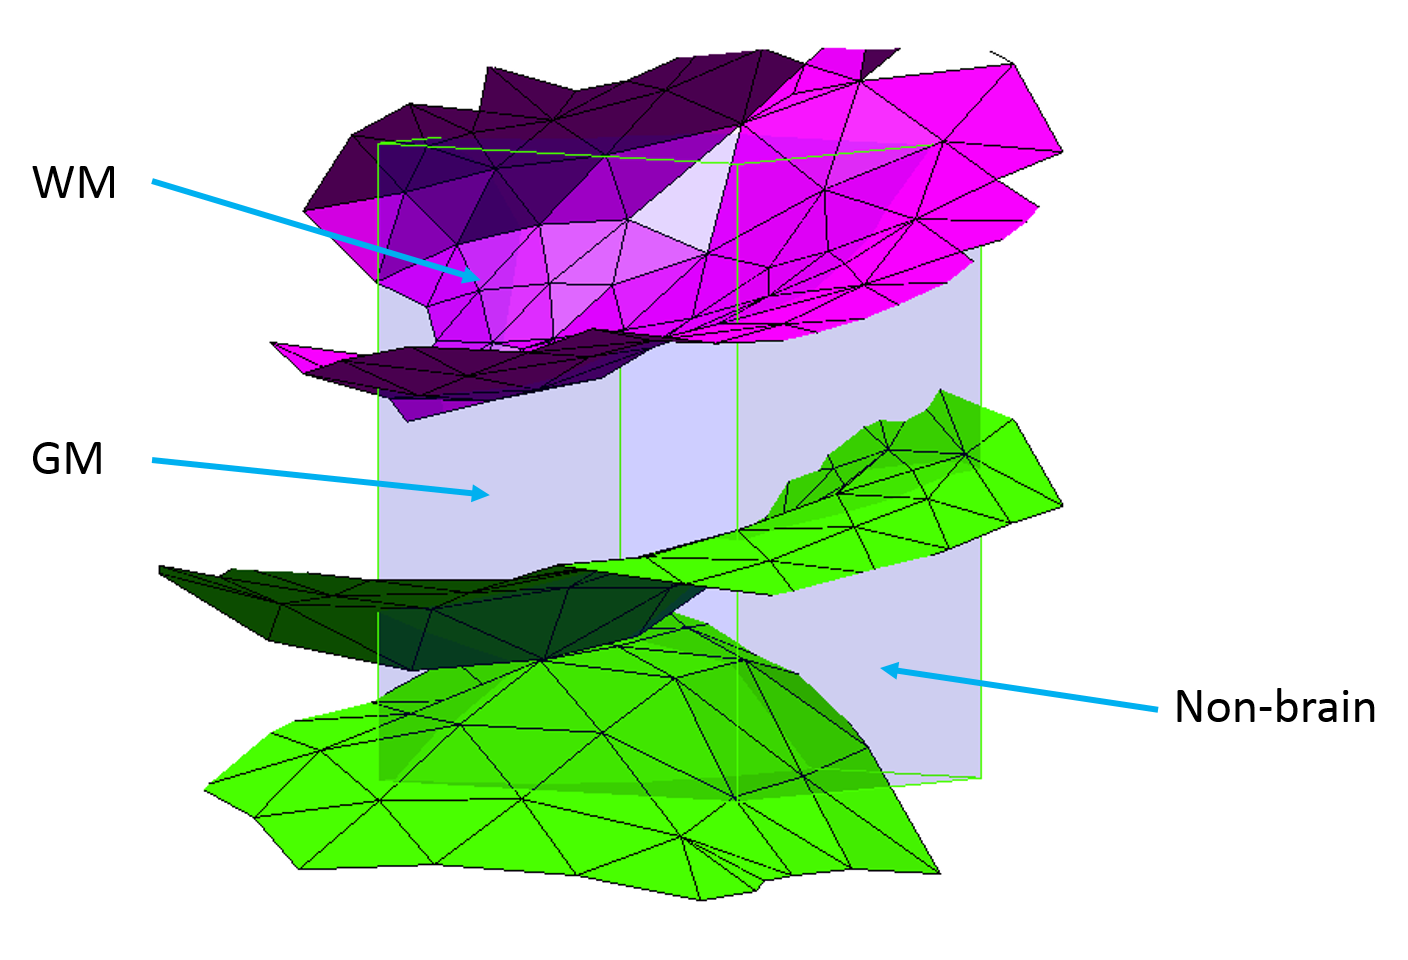
\includegraphics[width = 0.7\textwidth]{example_voxel.png}
\caption{Intersection of inner (magenta) and outer (green) surfaces of the cortex with a voxel. The outer surface intersects twice with distinct patches of surface; this is likely due to the presence of a sulcus. Tissue PVs are labelled.  }
\label{example_voxel}
\end{figure}

The first step is to identify and record the local patches of surface intersecting each voxel of the reference grid via Moller’s triangle-box overlap test \cite{Akenine-Moller2001}. The geometry of a surface within a voxel can frequently be complex: using a sulcus of the cortex as an example, the surface may intersect the voxel multiple times, with the opposite banks of the sulcus appearing as two unconnected patches of surface, illustrated in figure \ref{example_voxel}f. Accounting for the many possible surface/voxel configurations requires numerous specific tests that rapidly become excessively complex, so the approach taken in Toblerone is to divide and conquer each voxel as required. As the length scale of a voxel decreases, the complexity of the local surface configuration within the voxel will also decrease (for example, a sulcus is less likely to intersect the voxel multiple times). Each voxel of the reference image is therefore divided into a number of subvoxels which are processed individually. The subdivision factor has been set empirically as $\mathrm{ceil}(\vec{v} / 0.75)$ where $\vec{v}$ is the vector of voxel dimensions and 0.75 represents the lower limit of feature size found in the brain (in other contexts this parameter could be varied). Note that this subdivision factor transforms anisotropic voxels into approximately isotropic subvoxels,  which are processed according to the following framework. 

\begin{itemize}
\item If the subvoxel does not intersect the surface, it is assigned a single-class volume according to an interior/exterior classification of its centre. This is illustrated in figure \ref{all_subvoxels}a. 

\item If the subvoxel intersects the surface, then it contains interior and exterior PVs. One of these will be estimated using a convex hull (via the Qhull implementation \cite{Barber:1996:QAC:235815.235821}) if the geometry of the surface is favourable, as follows:

\begin{itemize}
\item If the surface intersects entirely through one face of the subvoxel, then it encloses a highly convex volume that may be reliably estimated. The other partial volume is calculated by subtraction from the total subvoxel volume. This is illustrated in figure \ref{all_subvoxels}b. 
\item If the surface is folded within the subvoxel (identified by multiple intersection of the surface along an edge or face diagonal of the subvoxel) then the subvoxel is subdivided a second time. This is because it is difficult to reliably identify which volume is interior or exterior in such a situation. This is illustrated in figure \ref{all_subvoxels}c/d. 
\item In all other cases, convex hulls are again used. In order to minimise the potential error associated with estimation of a non-convex volume via the use of a convex hull, it is important to identify which of the two PVs within the subvoxel is closer to being genuinely convex than the other. The proxy measure used for this is the number of subvoxel vertices lying on either side of the surface: the side with fewer vertices is assumed to enclose a more convex (and at any rate smaller) volume than the other. This is illustrated in figure \ref{all_subvoxels}e.
\end{itemize}

\item If the surface intersects the subvoxel multiple times (identified by the successful separation of surface vertices lying within the subvoxel into unconnected groups) then the voxel is subdivided a second time. This situation occurs for example when the opposite banks of a sulcus pass through a voxel. Although the reduced ray intersection test is accurate in such a situation, forming convex hulls is not, so subdivision is the safer option. This is illustrated in figure \ref{all_subvoxels}f. 
\end{itemize}

\begin{figure}
\centering
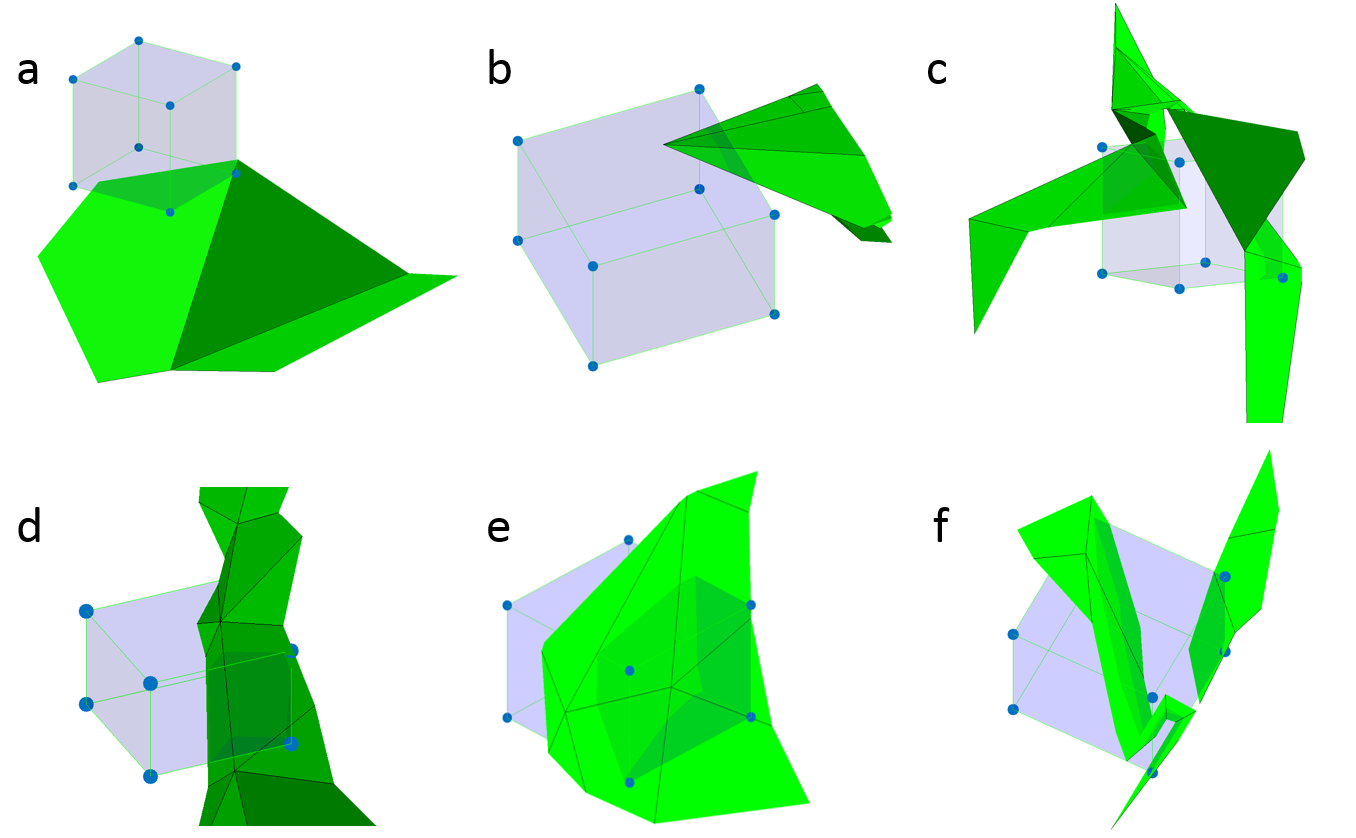
\includegraphics[width = \textwidth]{all_subvoxels.png}
\caption{Various subvoxel/surface configurations. a) no intersection: whole-volume assignment; b) single intersection through one face: a small convex hull will be formed; c/d) two examples of single intersection, folded surface: further subdivision will be used; e) single intersection through multiple faces: a convex hull will be formed; f) multiple surface intersection (unconnected patches of surface, likely a sulcus): further subdivision will be used. }
\label{all_subvoxels}
\end{figure}

If required, the second subdivision is performed at a constant factor of five to yield sub-subvoxels of approximately 0.1 to 0.2mm side length isotropic. These are always assigned a single-class volume based on a classification of their centre points as their small size means that any PVE will be negligible. Finally, voxels that do not intersect the surface (fully interior or exterior) are given single-class volumes according to tests of their centre points. Structures defined by a single surface (e.g. the thalamus) require no further processing: the estimates produced by the aforementioned steps may be used directly for PVEc.
 
\subsection{Estimation for multiple-surface structures}
Structures that are defined by multiple surfaces require further processing to yield PV estimates for all tissues of interest. Using the cortex as an example, PVs within each hemisphere are obtained with the following relations:

\begin{align}
PV_{WM} &= P_{inner} \\
PV_{GM} &= \mathrm{max}(0, P_{outer} - P_{inner}) \\
PV_{NB} &= 1 - (PV_{WM} + PV_{GM}) 
\end{align}

where $P_{inner}$ and $P_{outer}$ denote the interior/exterior PV fractions associated with the inner and outer surfaces of the cortex respectively and $PV_{WM}, PV_{GM}$ and $PV_{NB}$ denote the PV estimates for WM, GM and non-brain tissue (the latter including cerebrospinal fluid, CSF). These equations are structured to account for a potential surface defect whereby the surfaces of the cortex swap relative position (the inner lying exterior to the outer) around the corpus collosum. The structure of the above relations ($N$ surfaces leading to $N+1$ tissue classes) could easily be generalised to structures defined by more than two surfaces (for example, sublayers of the cortex, as used in laminar fMRI). A similar set of equations is used to merge hemisphere-specific results to cover the whole cortex, accounting for voxels lying on the mid-sagittal plane that intersect both hemispheres.
 
\subsection{Whole-brain PV estimation}
Toblerone, as outlined above, operates on a structure-by-structure basis in which the output tissue types are dependent on the structure in question. A number of methods utilising this core functionality have been implemented for general use cases: 
\begin{itemize}
	\item \textit{estimate\_structure}: estimate the interior and exterior PVs associated with a structure defined by a single surface
	\item \textit{estimate\_cortex}: estimate the GM, WM and non-brain PVs associated with the four surfaces of the cortex (l/r white/pial in the FreeSurfer terminology) 
	\item \textit{estimate\_all}: a combination of the structure and cortex methods above, this estimates PVs for the cortex and all subcortical structures identified by FIRST and combines them (with the exception of the brain stem) into a single set of GM, WM and non-brain PV estimates. 
\end{itemize}
The run-time for \textit{estimate\_all} running on the output of FreeSurfer and FSL FIRST for a single subject was around 20 minutes on a desktop machine; given the vector-heavy nature of the calculations involved, this could likely be reduced on GPU hardware. 
	
The combination of FreeSurfer/FIRST and Toblerone's \textit{estimate\_all} provides a complete pipeline for obtaining whole-brain PV estimates in an arbitrary reference voxel grid from a single T1-weighted image that may be used as a replacement for existing volumetric PV estimation tools such as FAST. There is however a key conceptual difference between surface and volumetric methods that concerns their interpretation of subcortical structures. Due to differences in tissue composition around the brain, cortical and subcortical GM typically have different intensities on a normal T1-weighted image (whereby cortical GM is seen as more ‘grey’ than subcortical, as illustrated in figure \ref{subcortical_gm_differences}). Being a histogram-based method, FAST will generally assign subcortical GM a lower GM PV estimate than might be expected as a result. In fact, by default FAST does not use any structural prior information and so is not even aware that these two different types of GM are in the same `class'; it simply determines subcortical GM to be more similar to cortical GM than it is to WM. 

Surface-based methods, by contrast, cannot take a nuanced view of the tissue composition of a subcortical structure. The surface that is used as input is treated as an absolute truth, with the implication that whatever tissue lies inside it is of a single type and is different to that outside. As a result, the tissue type of a structure must be determined using contextual or prior information (a conventional volumetric segmentation may be used to determine which tissue lies outside a structure). Thus, when combining the PVs of individual structures in Toblerone’s \textit{estimate\_all} function, it is necessary to know \textit{in advance} how the tissue type of each structure should be interpreted. In this work, all subcortical structures identified by FIRST (with the exception of the brain stem) were treated as pure GM. The practical implication of this is that Toblerone’s estimates for subcortical GM are higher than those produced by FAST (illustrated in figure \ref{subcortical_gm_differences}). For this reason, the conventional GM/WM/CSF tissue classes used by volumetric tools may be better thought of within Toblerone’s framework as tissue of interest, other tissues and non-brain, though for the purposes of this article the familiar names GM and WM shall be used alongside non-brain. The inherent ambiguity in determining which tissues lie outside subcortical structures, which could be either WM or CSF depending on their location within the brain, was resolved using FAST’s segmentation results.

\begin{figure}[H]
\centering
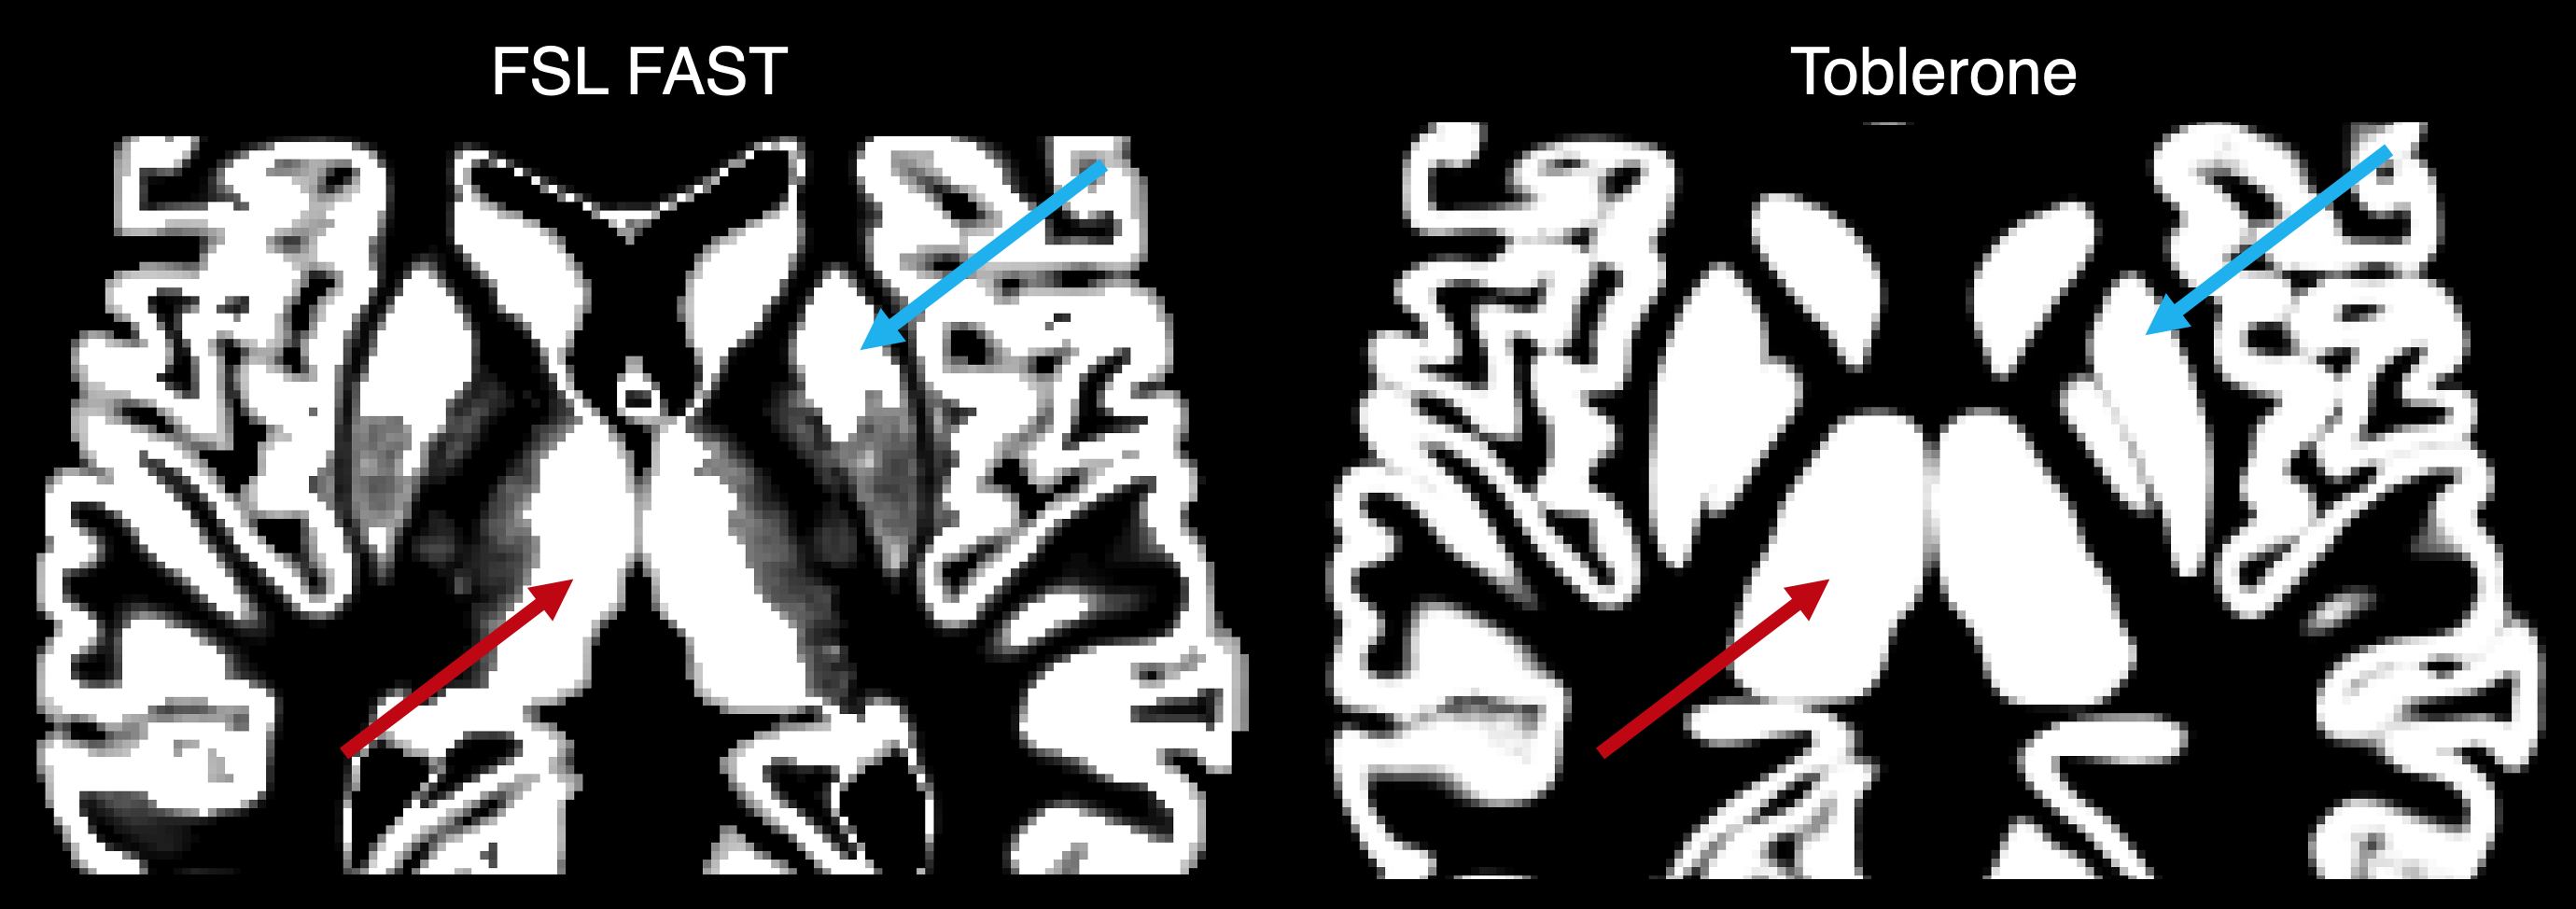
\includegraphics[width = \textwidth]{subcortical_gm_differences.png}
\caption{The left thalamus (red) and right putamen (blue) highlighted on the GM PV estimates of Toblerone and FAST on a typical subject, showing how surface and volumetric methods differ markedly in their interpretation of subcortical structures (FAST does not regard them as pure GM, whereas Toblerone does for the analyses presented in this work).}
\label{subcortical_gm_differences}
\end{figure}

\section{Methods}

\label{tob_pv_evaluation}

Three comparator methods were used to evaluate Toblerone. The two surface-based comparator methods were restricted to use in the cortex only as they cannot operate on subcortical structures defined by a single surface. Toblerone was run on both cortical and subcortical surfaces where possible to produce whole-brain PV estimates. 

The first surface-based comparator method, the ribbon-constrained (RC) algorithm, was developed for use with BOLD data in the HCP’s \textit{fMRISurface} pipeline \cite{Glasser2013} and is restricted to use in the cortex only. The method assumes vertex correspondence between the two surfaces of the cortex and works as follows. For each vertex in turn, the outermost edges of the triangles that surround that vertex are connected between the two surfaces to form a 3D polyhedron representing a small region of cortex. Nearby voxels are subdivided and the subvoxels centres tested to determine if they lie interior to the polyhedron. The subdivision factor used in this work was the higher value of either $\mathrm{ceil}( \mathrm{max} (\vec{v}/0.4) )$ or 4, where v is the vector of voxel dimensions. The fraction of subvoxel centres lying within any cortical polyhedron gives the cortical GM PV, which, as the BOLD signal is predominantly cortical in origin, is the quantity of interest for this modality. In order to obtain WM and non-brain PVs, the following post-processing steps were used. Firstly, the unassigned PV of each voxel was calculated as $1-PV_{GM}$, which was subsequently labelled as either WM or non-brain according to a signed-distance test of the voxel centre in comparison to the cortical mid-surface: for a voxel with centre point outside the mid-surface, the unassigned PV was labelled as non-brain. A weakness of this approach is that it is unable to faithfully capture a voxel in which all \textit{three} tissues are present; only the combinations WM/GM or GM/non-brain are permitted. As voxel size increases, the probability of voxels containing multiple tissues also increases; testing on an image of 3mm isotropic resolution showed that around 30\% of voxels intersecting the cortical ribbon contained three tissues. Resampling can be used to mitigate this effect so two variants of this method were tested: ‘RC’, direct estimation at each resolution, and ‘RC2’, estimation at 1mm followed by resampling to other resolutions via the process in section \ref{applywarp}. The run-time for a typical subject was around 15 minutes. 

The second surface method, NeuroPVE \cite{NeuropolyPVE}, is based on the voxelisation work of \cite{Nooruddin2003}, applied in a brain-specific context and again restricted to use in the cortex only. Multiple expanded and contracted copies of each cortical surface are created and the ratio of expanded to contracted surfaces intersecting a given voxel is used as a first approximation for partial volumes. This ratio is then mapped, along with surface orientation information, via trigonometric relations on the unit cube into a PV estimate. The estimates produced take discrete values according to the number of surfaces used (in this work the default of five). The intended use of this tool was PV estimation at structural, not functional, resolution, so two variants were tested: ‘Neuro’, direct estimation at arbitrary resolutions, and ‘Neuro2’, estimation at structural resolution followed by resampling to other resolutions via the process in section \ref{applywarp}. On the basis of NeuroPVE’s results on the simulated surfaces, it was excluded from further analysis. As the process of surface inflation is slow, the run-time for a typical subject was around 12 hours. 

Finally, FSL’s FAST \cite{Zhang2001} is an established whole-brain volumetric segmentation tool that was used as a comparator for the surface methods. On both the BrainWeb and HCP test-retest datasets, FAST was run on the brain-extracted images at structural resolution (1mm and 0.7mm isotropic respectively). PVs were then obtained at other resolutions via the resampling method detailed in paragraph \ref{applywarp}. The run-time for a typical subject was around five minutes. 

\subsection*{Resampling via applywarp}
\label{applywarp}
Resampling is an interpolation operation that is used to transform volumetric data between voxel grids (in this context, from structural to functional resolution). FSL’s \textit{applywarp} tool was used with the \textit{-super} flag for all resampling operations. This works by creating an up-sampled copy of the target voxel grid onto which values from the input image are sampled. The average is then taken across the voxel neighbourhoods of the high-resolution grid (sized according to the up-sampling factor) to obtain the result in the target voxel grid. Such an approach is appropriate when moving from fine to coarse as each output voxel corresponds to multiple input voxels, the individual contributions of which should be accounted for to preserve overall tissue proportions. When using \textit{applywarp} a transformation matrix between the input and output voxel grids must be given as the \textit{-premat} argument; to denote identity for the purposes of this work, the output of the HCP \textit{wb\_command –convert-affine –from-world –to-flirt} tool operating on the identity matrix $\mat{I}_4$ was used as the \textit{-premat} to correct for a subvoxel shift that arises due to FSL coordinate system conventions. Note that for perfectly aligned voxel grids with an integer ratio of voxel sizes, such as a 1mm and 2mm isotropic grid, this process is equivalent to averaging across blocks of the smaller grid (sized 2x2x2 in this case).

\section{Datasets}

Four datasets were used to evaluate Toblerone. Three of these pertained to PV estimation specifically, as summarised in table \ref{tob_datasets}, and the final one investigated the link between PV estimates and PVE in physiological data.

\begin{table}[H]
\setlength{\tabcolsep}{0.75em} % for the horizontal padding
{
    \renewcommand{\arraystretch}{1.2}% for the vertical padding
    \begin{tabular}{p{2.5cm}|p{3.5cm}p{3.5cm}p{3.6cm}}
    \textit{name} & Simulated surfaces & BrainWeb & HCP test-retest \\ \cline{1-4}
    \textit{type} & S & V \& S & V \& S \\
    \textit{resolution} & - & 1mm iso. & 0.7mm iso. \\
    \textit{size} & \begin{tabular}[c]{@{}l@{}}one cortical \\hemisphere \end{tabular} & \begin{tabular}[c]{@{}l@{}}one subject, \\18 structural images\end{tabular} & \begin{tabular}[c]{@{}l@{}}45 subjects,\\2 structural images each\end{tabular} \\
    \textit{ground truth} & numerical method & volumetric segmentation* & N/A \\
    \textit{comparator methods} & \begin{tabular}[c]{@{}l@{}}NeuroPVE (S)\\ RC (S)\end{tabular} & \begin{tabular}[c]{@{}l@{}}RC** (S)\\ FAST (V)\end{tabular} & \begin{tabular}[c]{@{}l@{}}RC** (S)\\ FAST (V)\end{tabular}
    \end{tabular}
}
\caption{Overview of methods and datasets used for evaluation of PV estimation. Key: S: surface, V: volumetric, RC: ribbon-constrained. 
* established via automatic segmentation with manual intervention. ** RC can only operate on the cortex, not subcortex, for these datasets.}
\label{tob_datasets}
\end{table}

\subsection{Simulated surfaces}
\label{tob_sim_surfaces}
A pair of concentric surfaces, illustrated figure \ref{simsurfs}, were designed to capture geometric features relevant to the anatomy of a cortical hemisphere. These were produced by modulating the radius of a sphere as a function of azimuth $\theta$ and elevation $\phi$ to produce sulcal and gyral-like features. The radius of the inner surface was defined as

\begin{equation}
r_{in} = 60 (1 - 0.1 \mathrm{max}(\sin^{20}(5u), \sin^{20}(5v) ) )
\end{equation}

where 60 is the unmodulated radius of the sphere, 0.1 fixes the relative depth of sulci, the max function prevents sulci from constructively interfering to produce deep wells at points of intersection, the power of 20 produces broad gyri and narrow sulci, and the substitutions $u= \phi + \theta$, $v= \phi - \theta$ cause the sulci to spiral around the sphere in opposite directions. Modulation was restricted to the range $-2\pi/5 \leq \theta \leq 2\pi/5$ to leave the poles smooth and suppress unrealistic features. The outer radius was set at $r_{out}= 1.05 \cdot r_{in}$, leading to a peak radial distance between surfaces of 3mm. The outermost region was taken to represent non-brain tissue, the innermost WM and the region in between GM. The use of analytic functions to define the surfaces permitted ground truth to be calculated using the following numerical method. Voxels were sampled at 4,096 elements per mm\textsuperscript{3} and the positions of these sample points expressed in spherical polar coordinates. By comparing the actual radius of each point to the calculated radius of the surface boundaries for the same azimuth and elevation, the tissue type of the sample point within the structure could be determined, and from there PVs obtained by aggregating results within voxels. This is referred to as the ‘numerical solution’ in the results section. All surface methods were used on this dataset to obtain PVs at voxel sizes of 1 to 3mm in steps of 0.2mm isotropic. 

\begin{figure}
\centering
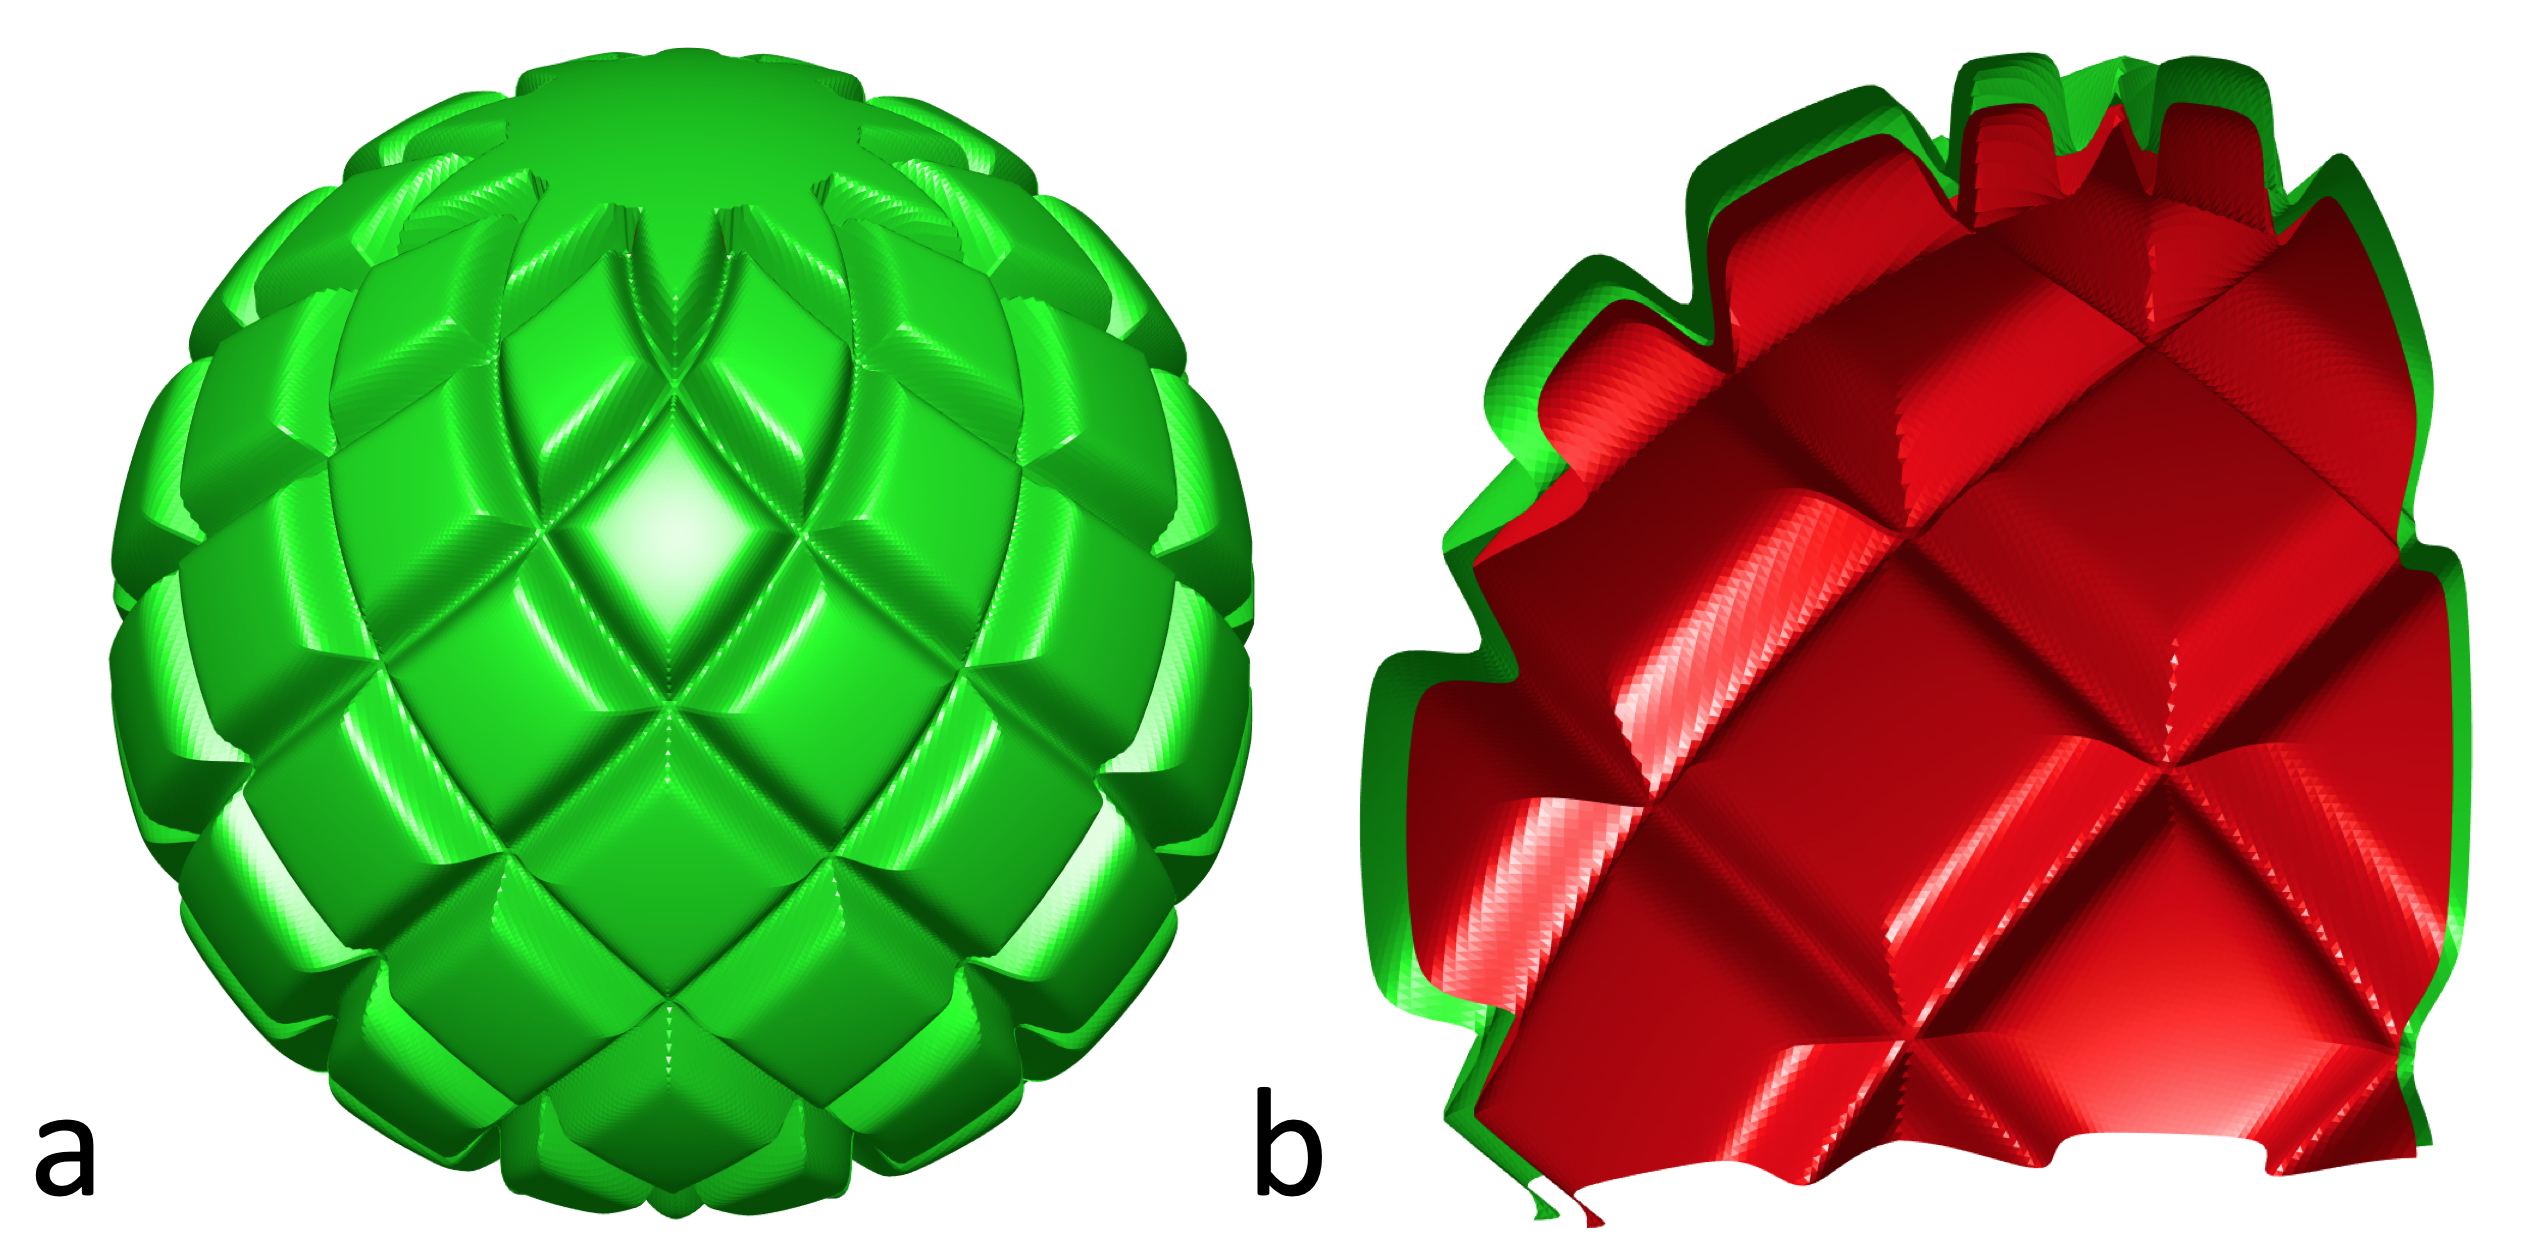
\includegraphics[width = 0.7\textwidth]{simsurfs.png}
\caption{a) Simulated surfaces; b) cutaway showing inner (red) and outer (green) surfaces. Peak radial distance between the two was 3mm.}
\label{simsurfs}
\end{figure}

\subsection{BrainWeb simulated T1 images}
BrainWeb \cite{Collins1998, Cocosco1997} simulates whole-head T1 images at 1mm isotropic resolution with specified levels of random noise and field non-uniformity (NU).  Eighteen images were produced to cover the available parameter space of noise levels 0, 1, 3, 5, 7, 9 and NU levels 0, 20, 40 (both quantities in percent). These were run through FIRST and FreeSurfer, after which Toblerone’s \textit{estimate\_all} and the RC method (cortex only) were used on the output. FAST was also used to enable a comparison between surface and volumetric methods. PVs were obtained at voxel sizes of 1 to 4mm in steps of 1mm isotropic. Although ground truth PV maps exist for this dataset (produced by automatic volumetric segmentation of T1 images with manual correction), both surface and volumetric methods returned significantly different results to these, raising the complicated question of determining which set of results is correct. In order to avoid making this judgement, each method was instead referenced to its own results on the ideal T1 image (0\% noise 0\% NU) in the 1mm isotropic voxel grid of the structural images; the objective of the test was to measure self-consistency across differing levels of noise and NU. The voxel grids associated with each voxel size were aligned such that results at 1mm could be used to calculate a reference at other sizes without resampling. 

\subsection{Human Connectome Project test-retest data} 
This dataset comprises 45 subjects from the main HCP cohort who underwent two separate structural scan sessions (mean age 30.2 years, mean time between sessions 4.8 months). Each session was processed using the pipeline in \cite{Glasser2013} to obtain cortical surfaces via FreeSurfer. Separately, the distortion-corrected T1 images were processed using FIRST to obtain subcortical surfaces. Toblerone’s \textit{estimate\_all} and the RC method (for the cortex only) were used on this dataset, as well as FAST for a comparison between surface and volumetric methods. PVs were obtained at voxel sizes of 1 to 3.8mm in steps of 0.4mm isotropic, as well as the native 0.7mm isotropic voxel grid of the structural images. As a ground truth is not defined for this dataset, each method’s results from the first session were used as a reference for the second session to permit self-consistency to be assessed. 

\subsection{\textit{In-vivo} ASL data} 
This dataset consists of ASL data at 1.5mm isotropic resolution from four subjects. For three subjects, four within-session repeats of 100 volumes were acquired; for the final subject a single repeat of 200 volumes was acquired. Other parameters were as follows: pASL FAIR QUIPSS-II at 7T field strength with a 2D EPI ascending readout, 32ms slice time, 1.8s TI, 700ms bolus duration and 0.95 inversion efficiency. Further details are given in appendix \ref{7T_appendix}. The data was downsampled without interpolation to 3mm isotropic resolution by summing across 2x2x2 voxel neighbourhoods to improve SNR and increase PVE. A T1w MP2RAGE structural image at 0.7mm isotropic resolution was obtained for each subject; these were processed to yield PV estimates from both the combined FreeSurfer/FIRST/Toblerone pipeline and FAST. CBF quantification was performed without PVEc using the \textit{oxford\_asl} pipeline \cite{Chappell2009, oxford-asl}; a T1 blood value of 2.2s \cite{Zhang2013} and voxel-wise calibration were used. The ASL data was analysed in native acquisition space; MCFLIRT and FLIRT \cite{flirt} were used to motion correct the data and register the T1w image to the ASL for the purpose of generating PV estimates in native space. EPI distortion correction was not performed, which would be expected to lead to areas of mis-alignment between the ASL data and the PV estimates; however due to the global nature of the analysis, the errors arising from this omission should be somewhat mitigated. The reader may refer back to figures \ref{ss_slices} and \ref{02_slices} to inspect the extent of distortion-induced misalignment. 

\subsection{Evaluation metrics}

For the PV estimation datasets, errors were measured in both a per-voxel (RMS of individual voxel errors) and aggregate (total tissue volume) sense. The former basis is important as PVEc is locally sensitive to the PV estimates \cite{Zhao2017a}; the latter basis reflects systematic bias at the aggregate level. All errors are expressed in percent and map directly to PV estimates without scaling: for example, a PV estimate of 0.5 against a reference value of 0.55 corresponds to an error of -0.05 or -5\%. Note that for some datasets where ground truth was not available, errors were measured with respect to each method's reference result (outlined earlier for each dataset). 

A further analysis of voxel-wise differences between Toblerone and FAST was performed on the HCP dataset at multiple voxel sizes by sorting voxels into 5\% width bins according to their Toblerone GM PV estimate. The difference (Toblerone – FAST) was calculated for each voxel and the mean taken across each bin. This quantity was then averaged across subjects and sessions (weighted to respect differences in brain volume).

For the \textit{in-vivo} ASL dataset only, linear regressions of non-PVEc CBF against GM PV were performed to assess the strength of the relationship between CBF and PV; theoretical understanding suggests this should be positive and approximately linear. Voxels containing at least 10\% GM PV on both Toblerone's and FAST's outputs were selected; using the intersection of both methods ensured that neither method was penalised in areas where they fundamentally disagreed about what tissues are present (notably, around some subcortical structures identified by FIRST). For the same reason, two separate regressions were performed: one with both cortical and subcortical GM, and the other considering the cortex only. The metric of interest in this analysis was the correlation coefficient ($R$ value); higher values imply that the PV estimates better explain the variation observed in the CBF data (which was known ahead of time to be corrupted by PVE). 

\section{Results}

\subsection{Simulated surfaces}

\begin{figure}[H]
\centering
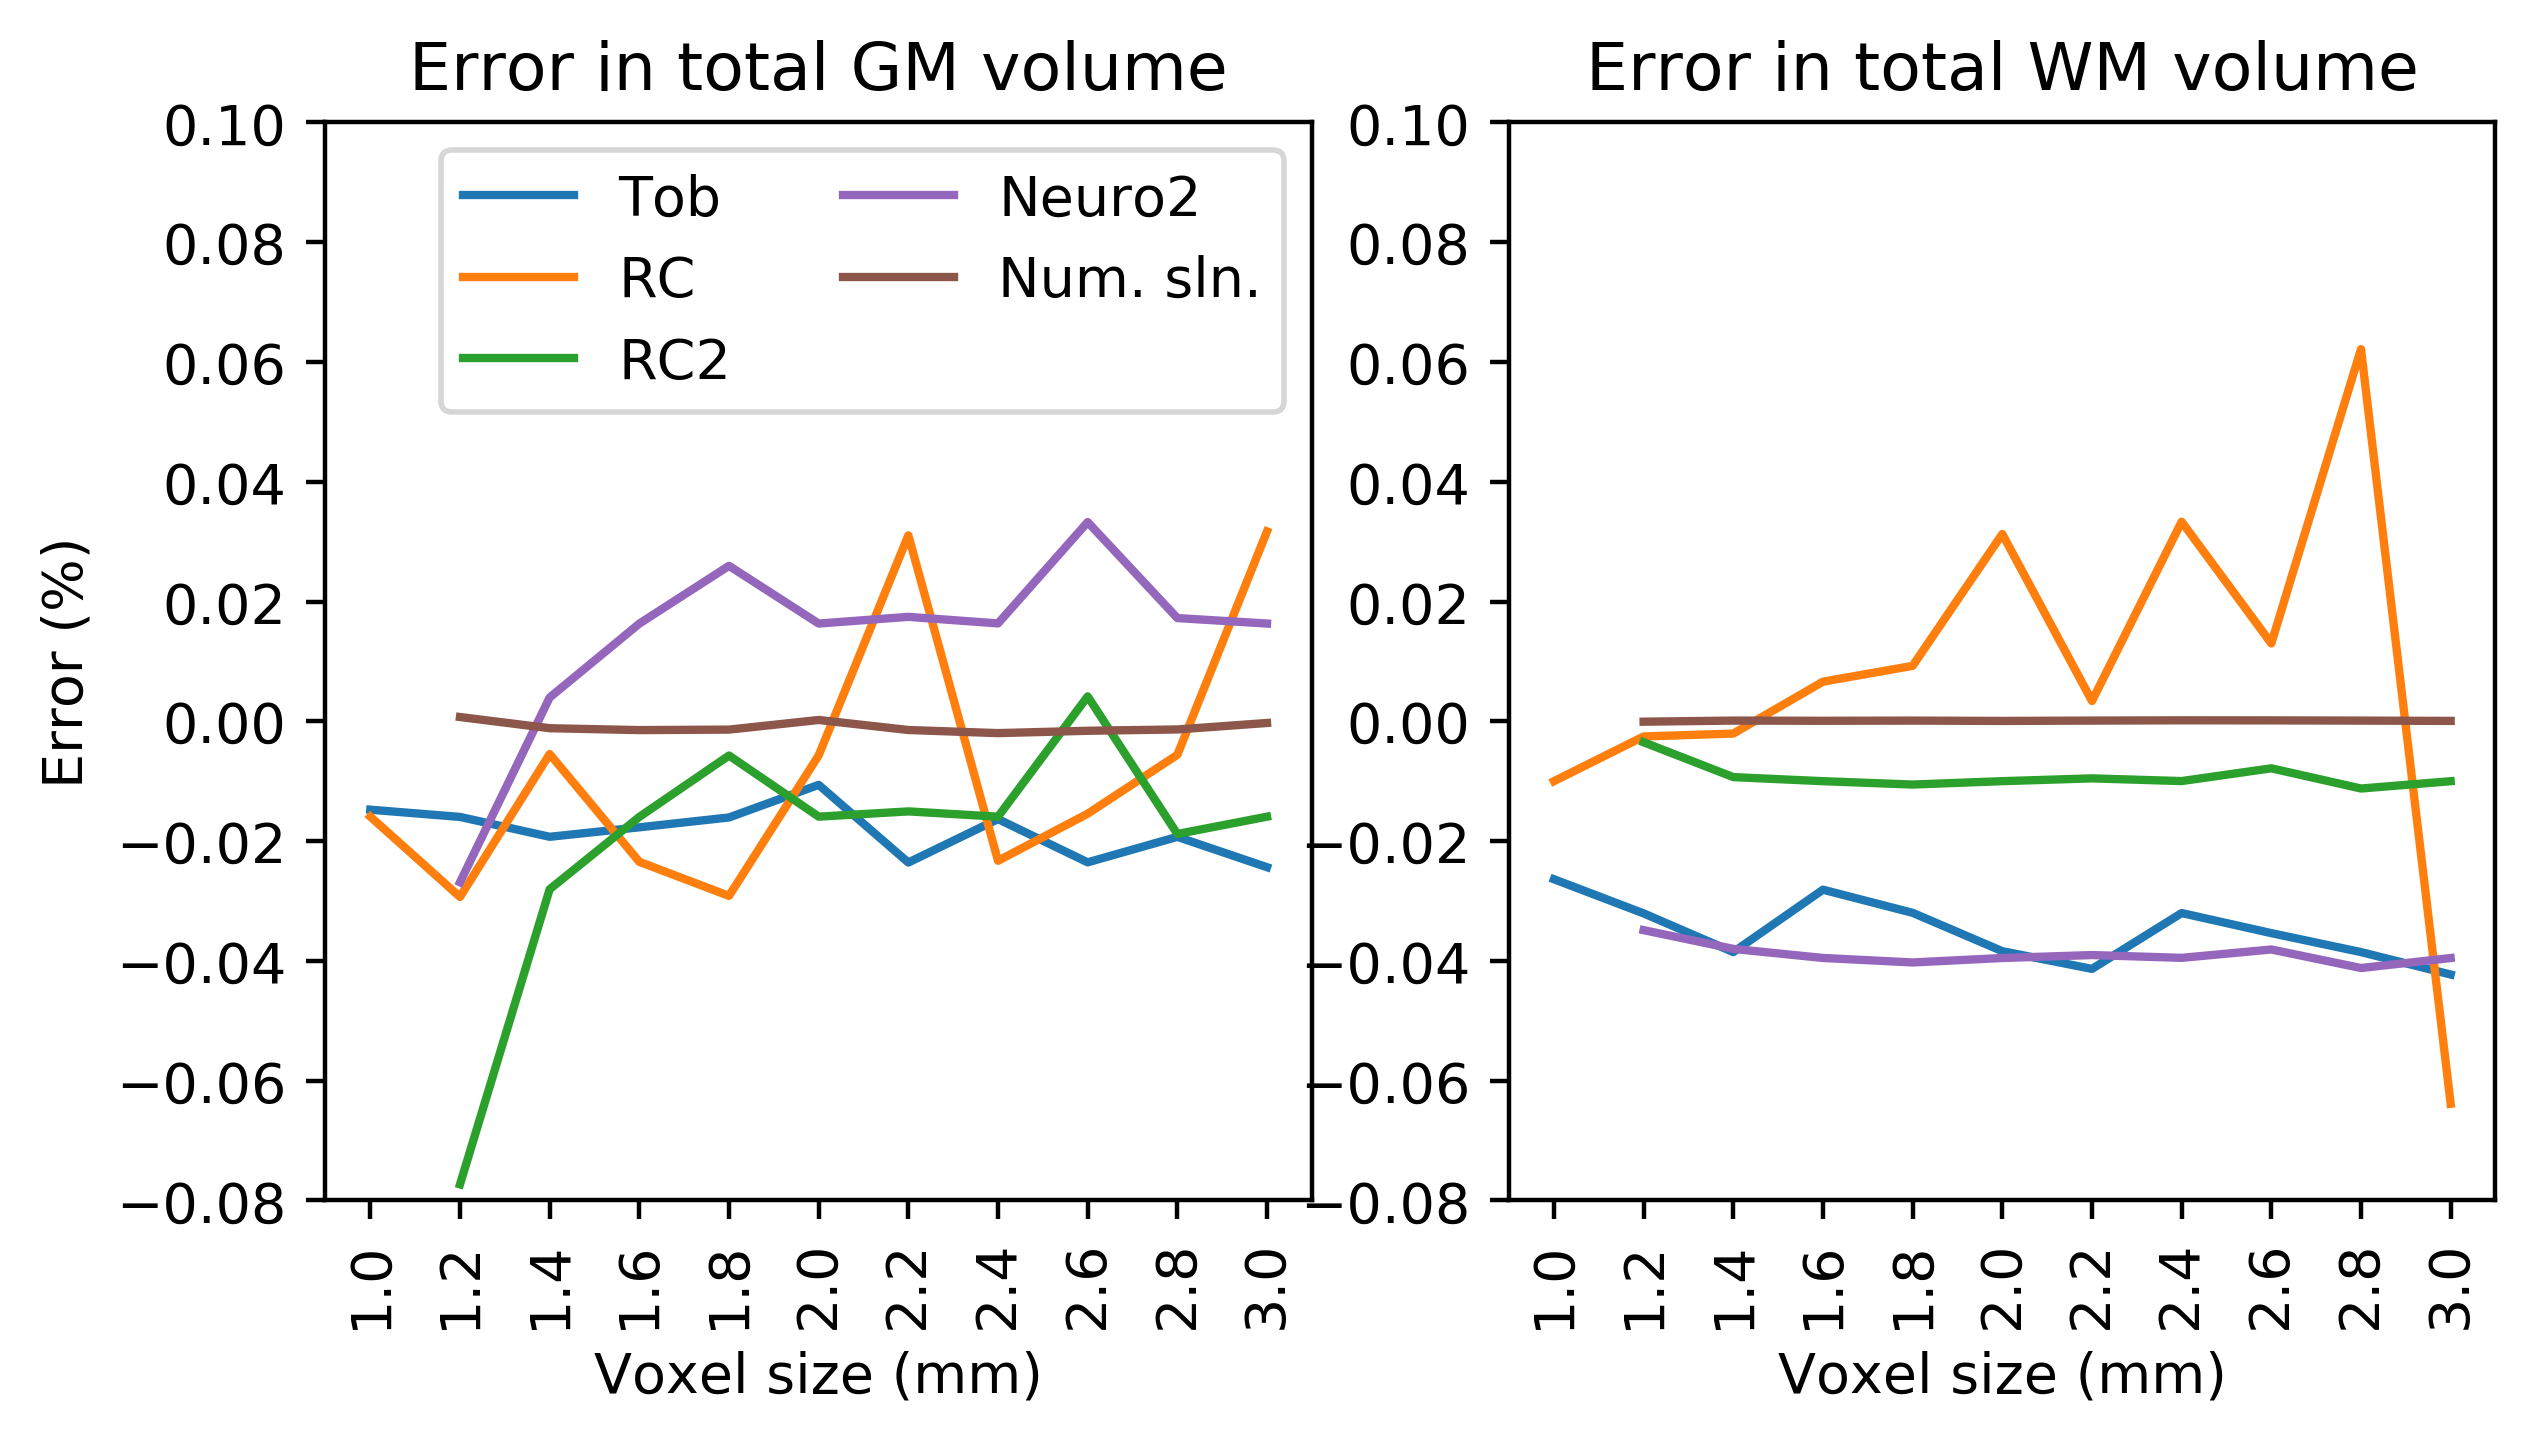
\includegraphics[width = 0.8\textwidth]{tob_sim_total.png}
\caption{Simulated surfaces: error in total tissue volume across all voxels, used to investigate bias and consistency across voxel sizes. Toblerone showed consistency, though with small bias, for both GM and WM. RC1 errors were lower for GM than WM. Resampling-based methods (RC2, Neuro2) showed particular consistency in WM. [Full results are in the appendix, figure \ref{tob_sim_total_supp}]}
\label{tob_sim_total}
\end{figure}

Figure \ref{tob_sim_total} shows the error in total tissue volume across all voxels for the simulated surfaces. The numerical solution at 1mm was used as the reference. Toblerone showed consistency across voxel sizes, though with a small negative bias in both GM and WM. RC estimates showed variation in both. The resampling-based methods RC2 and Neuro2 showed high consistency in WM but less so in GM. The numerical solution was stable across voxel sizes. Neuro’s results are excluded from this and subsequent graphs for clarity; the full results are given in the appendix, figure \ref{tob_sim_total_supp}). 

\begin{figure}[H]
\centering
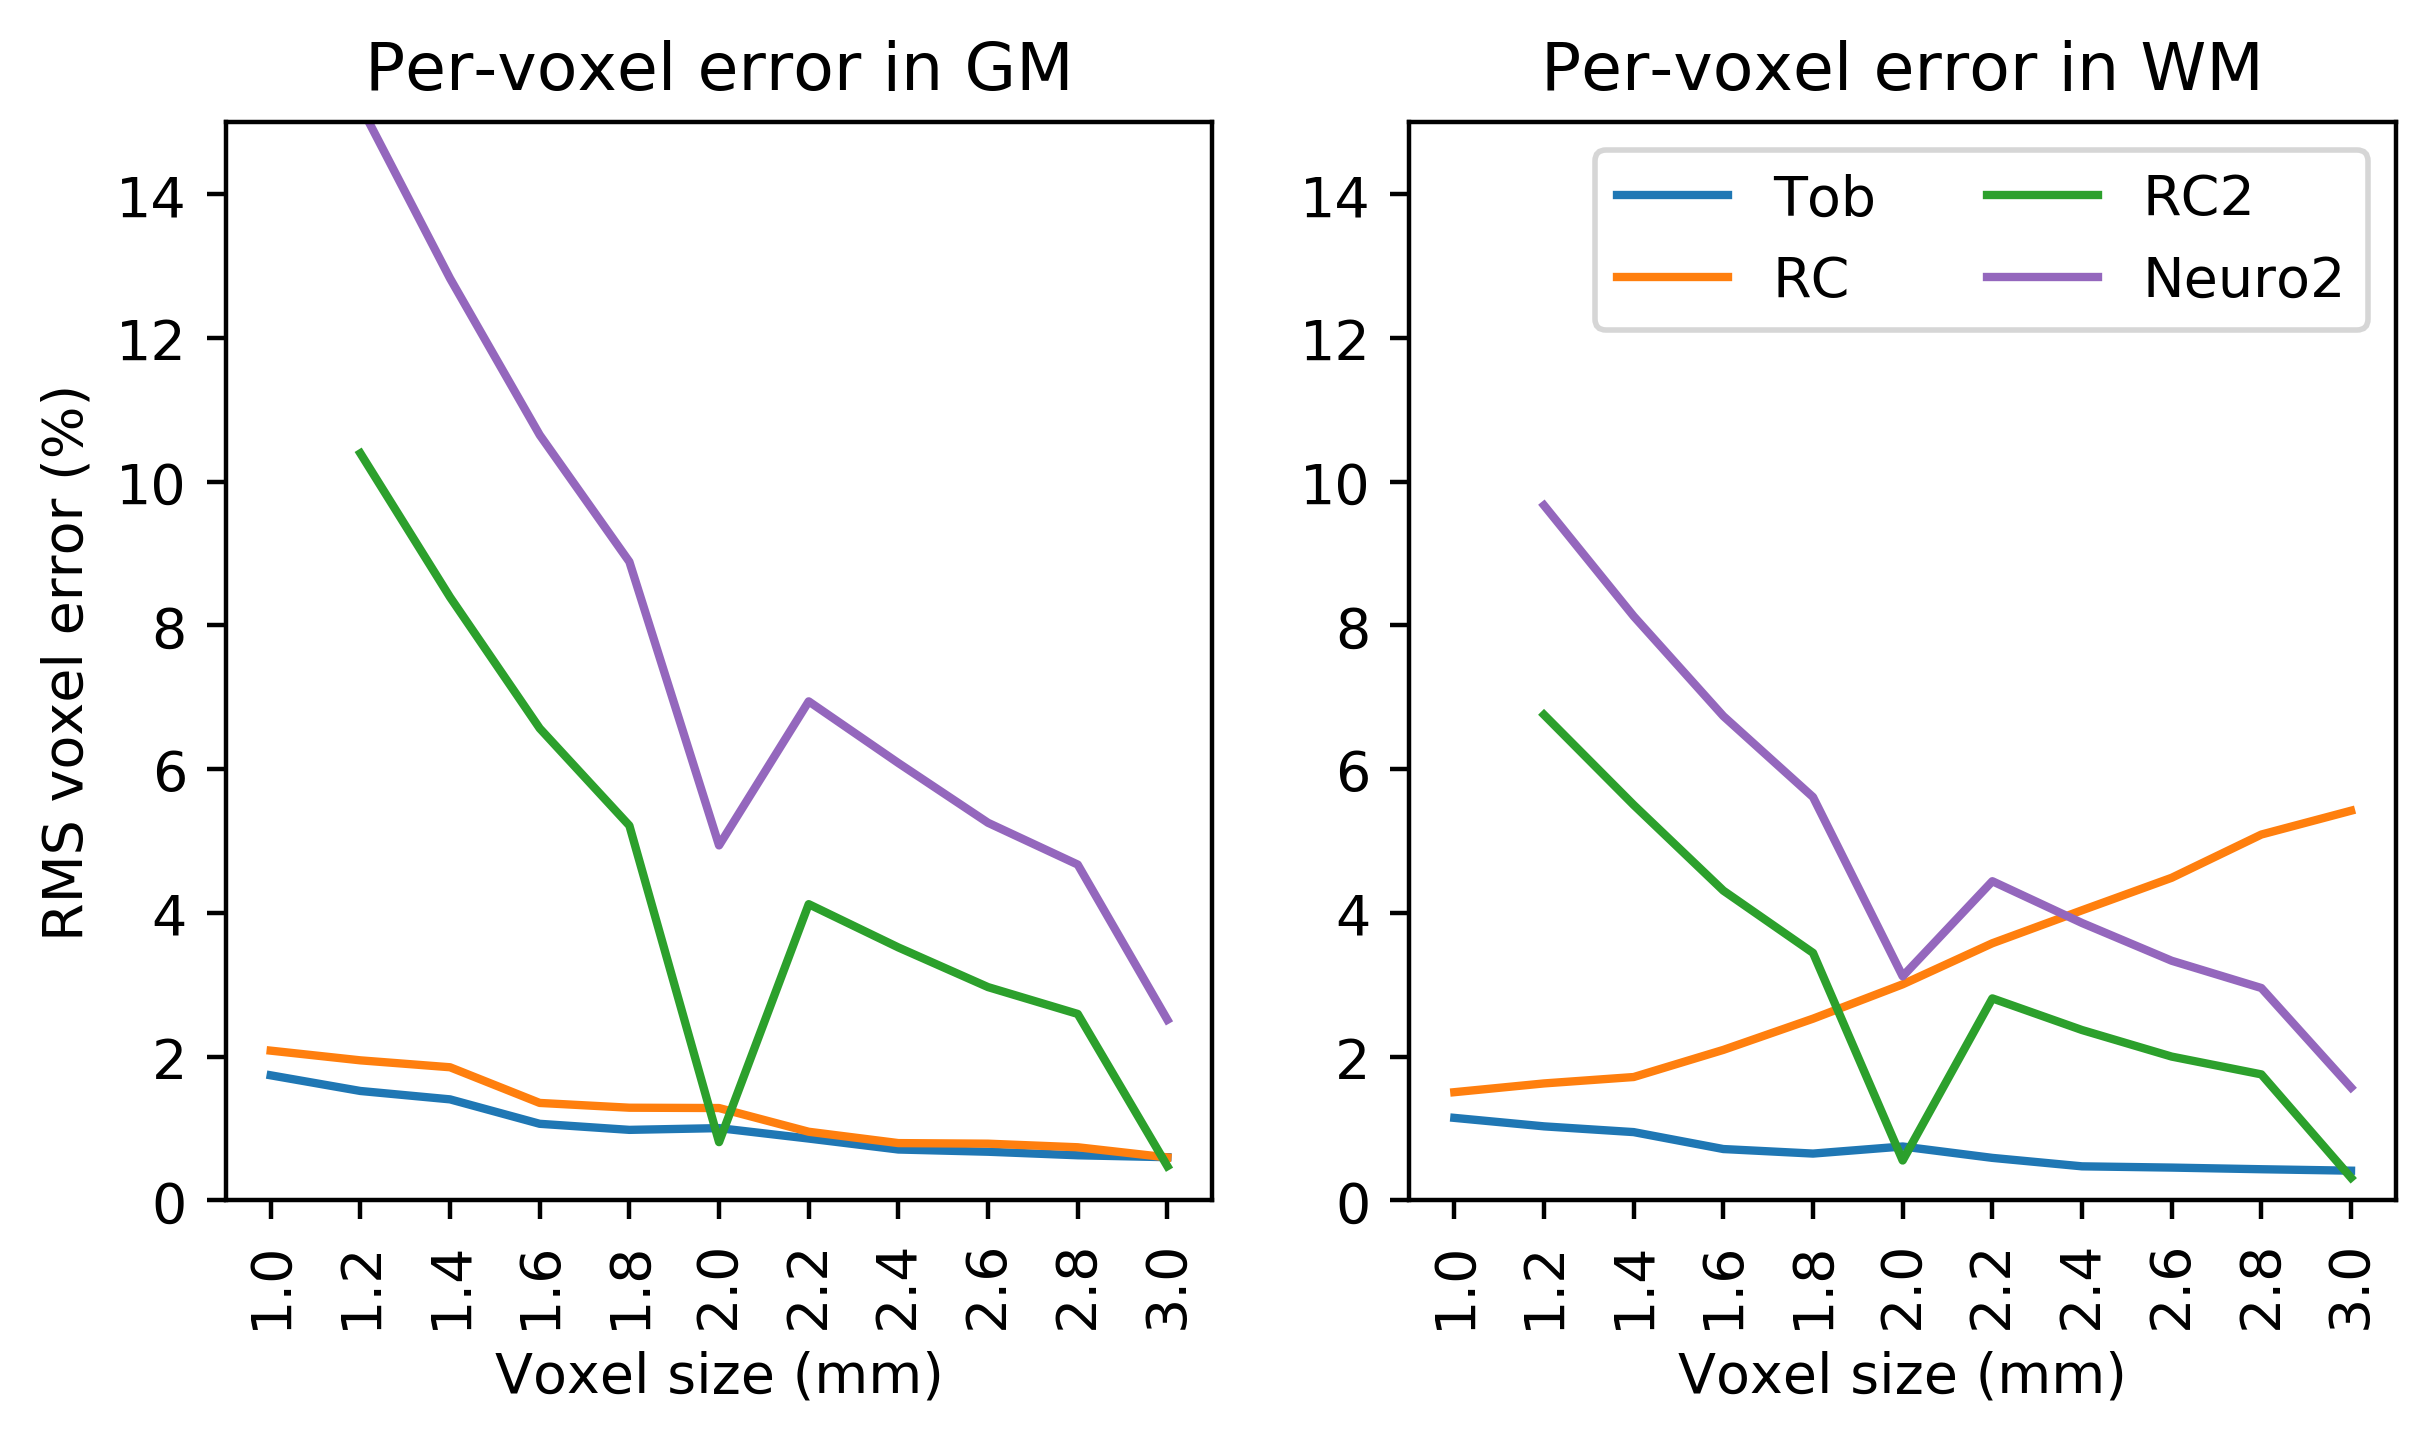
\includegraphics[width = 0.8\textwidth]{tob_sim_voxel.png}
\caption{Simulated surfaces: per-voxel error. Toblerone and RC produced the lowest errors in GM; in WM there was a clear difference to Toblerone. RC2 and Neuro2’s errors both decreased with increasing voxel size, with a characteristic notch observed at 2mm. [Full results are in the appendix, figure \ref{tob_sim_voxel_supp}]}
\label{tob_sim_voxel}
\end{figure}

Figure \ref{tob_sim_voxel} shows per-voxel error for the simulated surfaces. Results were masked to consider voxels intersecting either surface of the cortex as only these contain PVs. Toblerone and RC produced the lowest errors at all voxel sizes in GM; in WM only Toblerone retained this behaviour. Resampling-based methods (RC2, Neuro2) produced lower errors as voxel size increased, and a characteristic notch in their results was observed at 2mm. Although RC initially performed better than RC2 in WM, the inverse was true above 2mm voxel size.

\subsection{BrainWeb}

\begin{figure}[H]
\centering
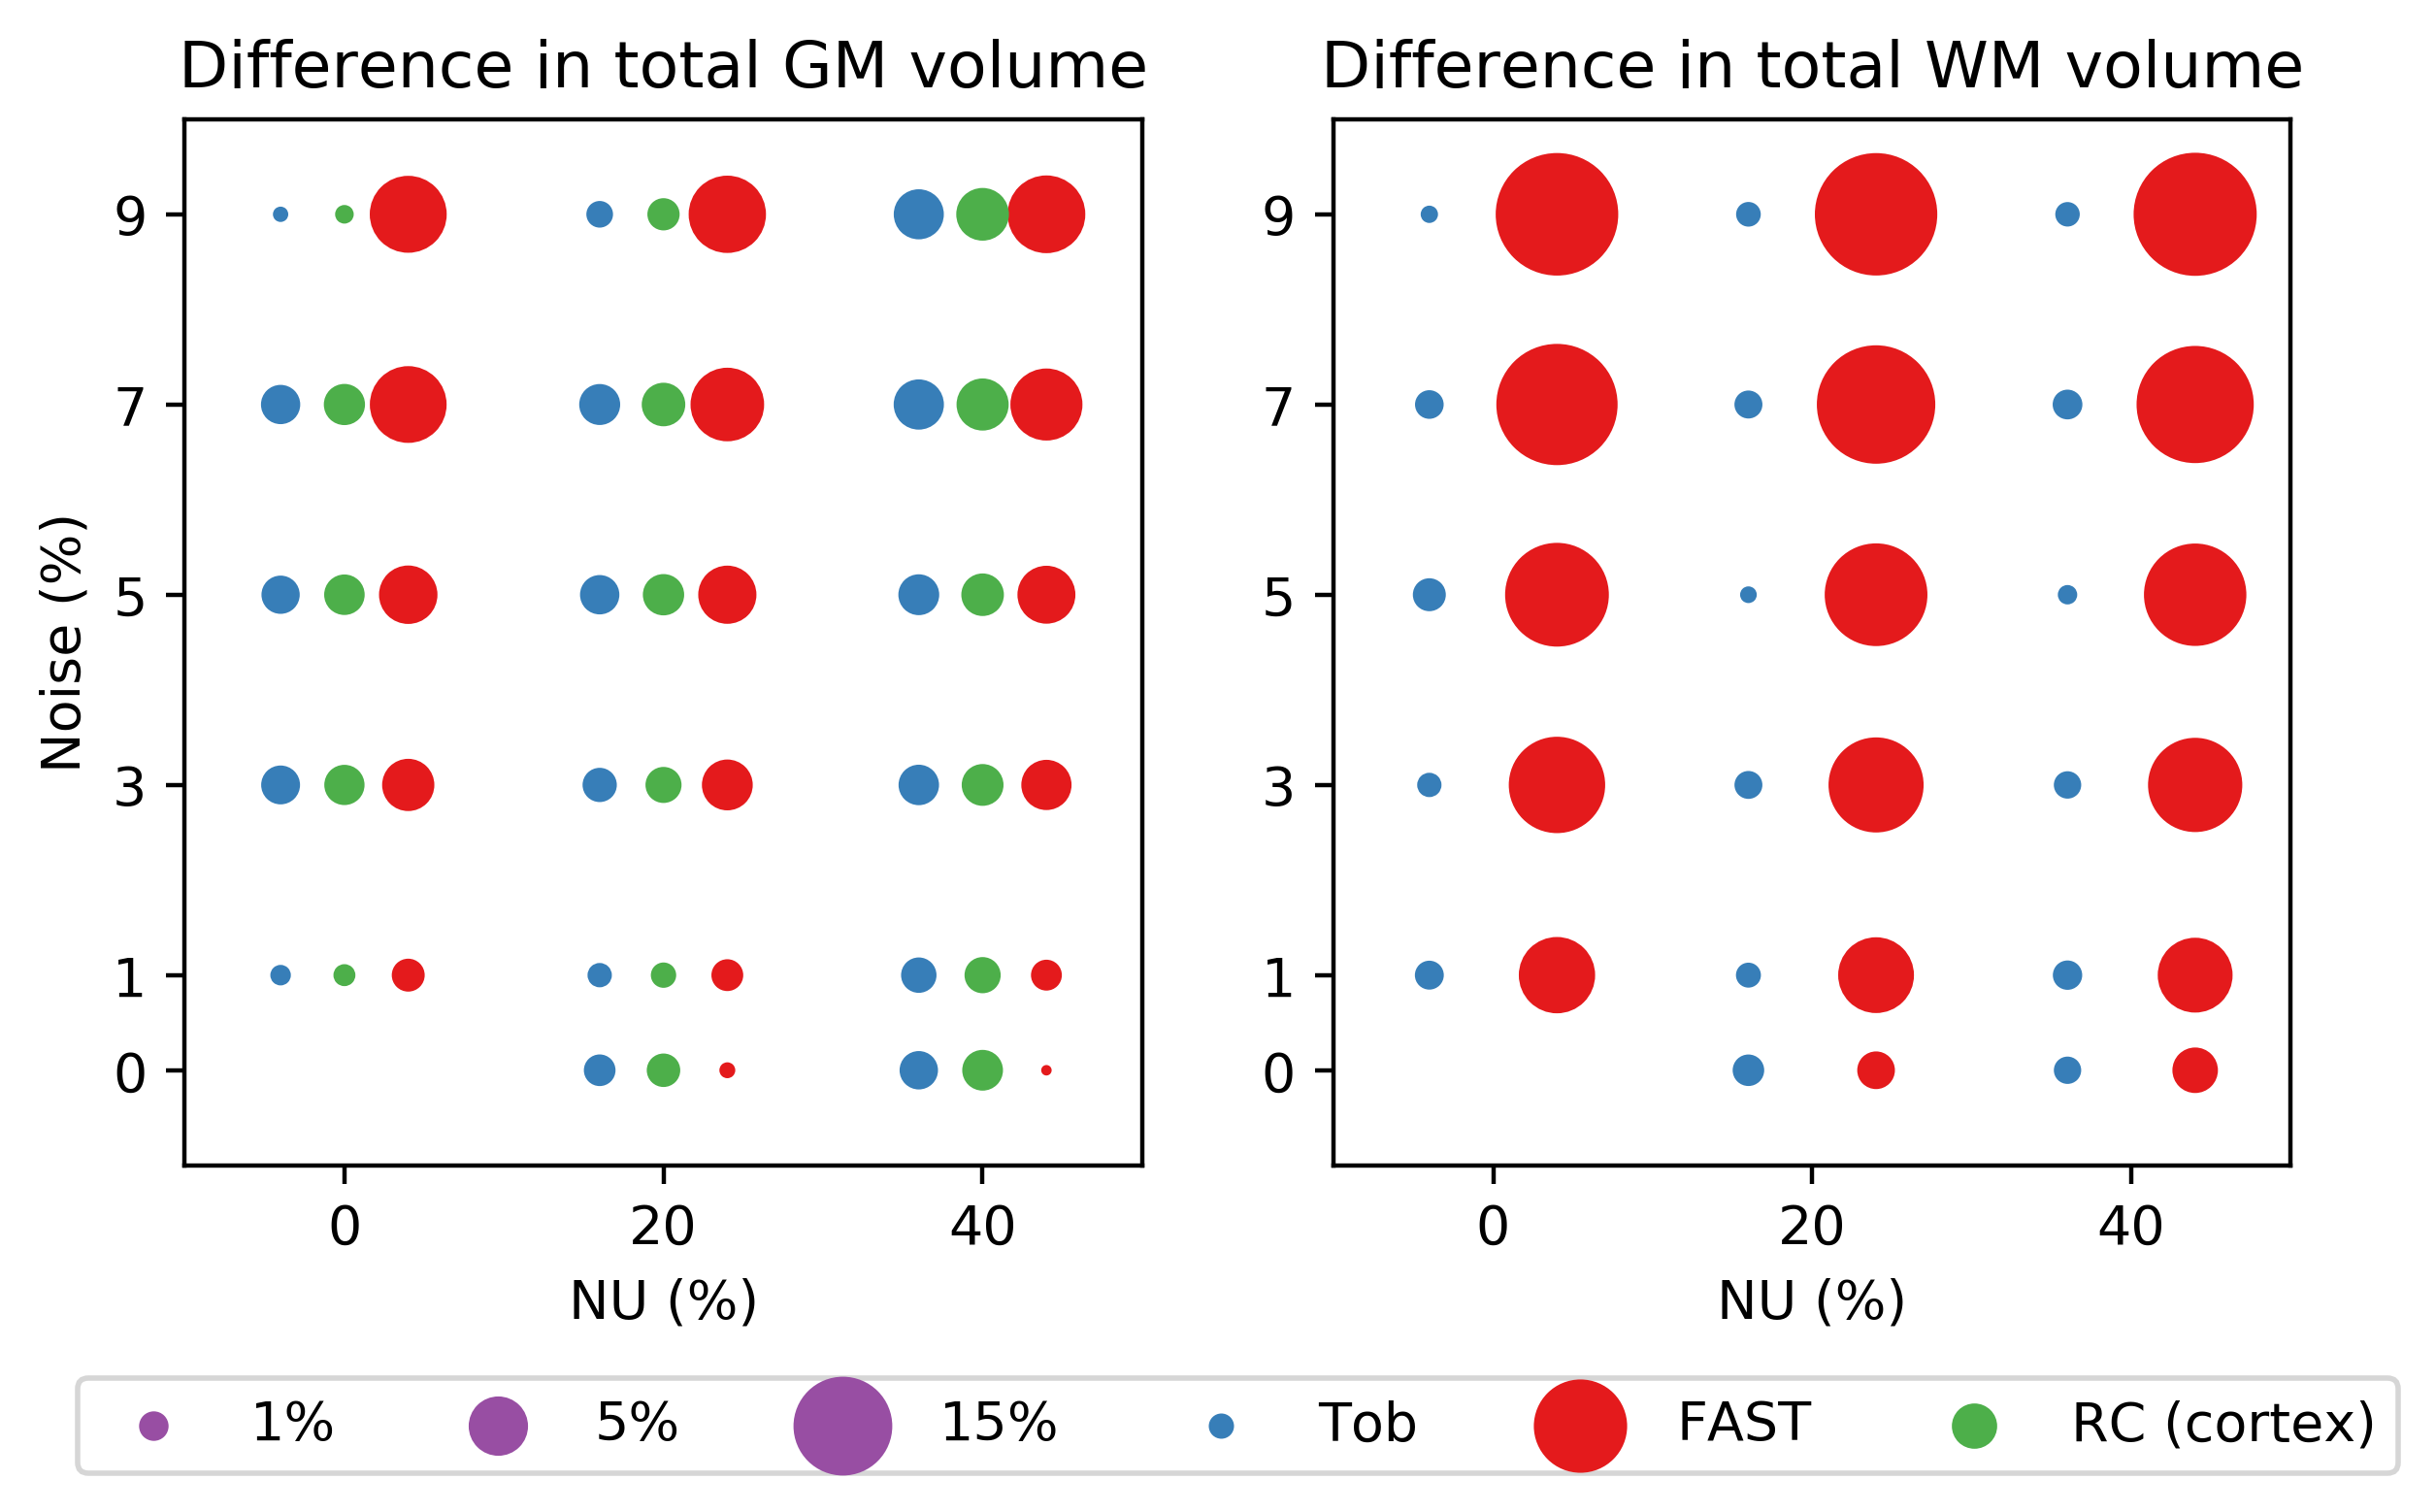
\includegraphics[width = 0.8\textwidth]{brainweb_total.png}
\caption{BrainWeb: difference in total tissue volume referenced to each method’s 0\% noise 0\% NU result. Surface-based methods were more consistent at almost all noise and NU levels; FAST was more consistent in GM than WM.}
\label{brainweb_total}
\end{figure}

Figure \ref{brainweb_total} shows the difference in total tissue volume for the BrainWeb phantom as a function of noise and NU levels, referenced to each method’s results at 0\% noise and 0\% NU. PV estimates at 1mm isotropic voxel size were used for this analysis. RC’s GM result was for the cortex only as it cannot process subcortical structures. In general, the surface-based methods showed more consistency in their estimates across all levels of noise and NU, with the notable exception of GM at 0\% noise. FAST’s consistency was notably better in GM than WM.

\begin{figure}[H]
\centering
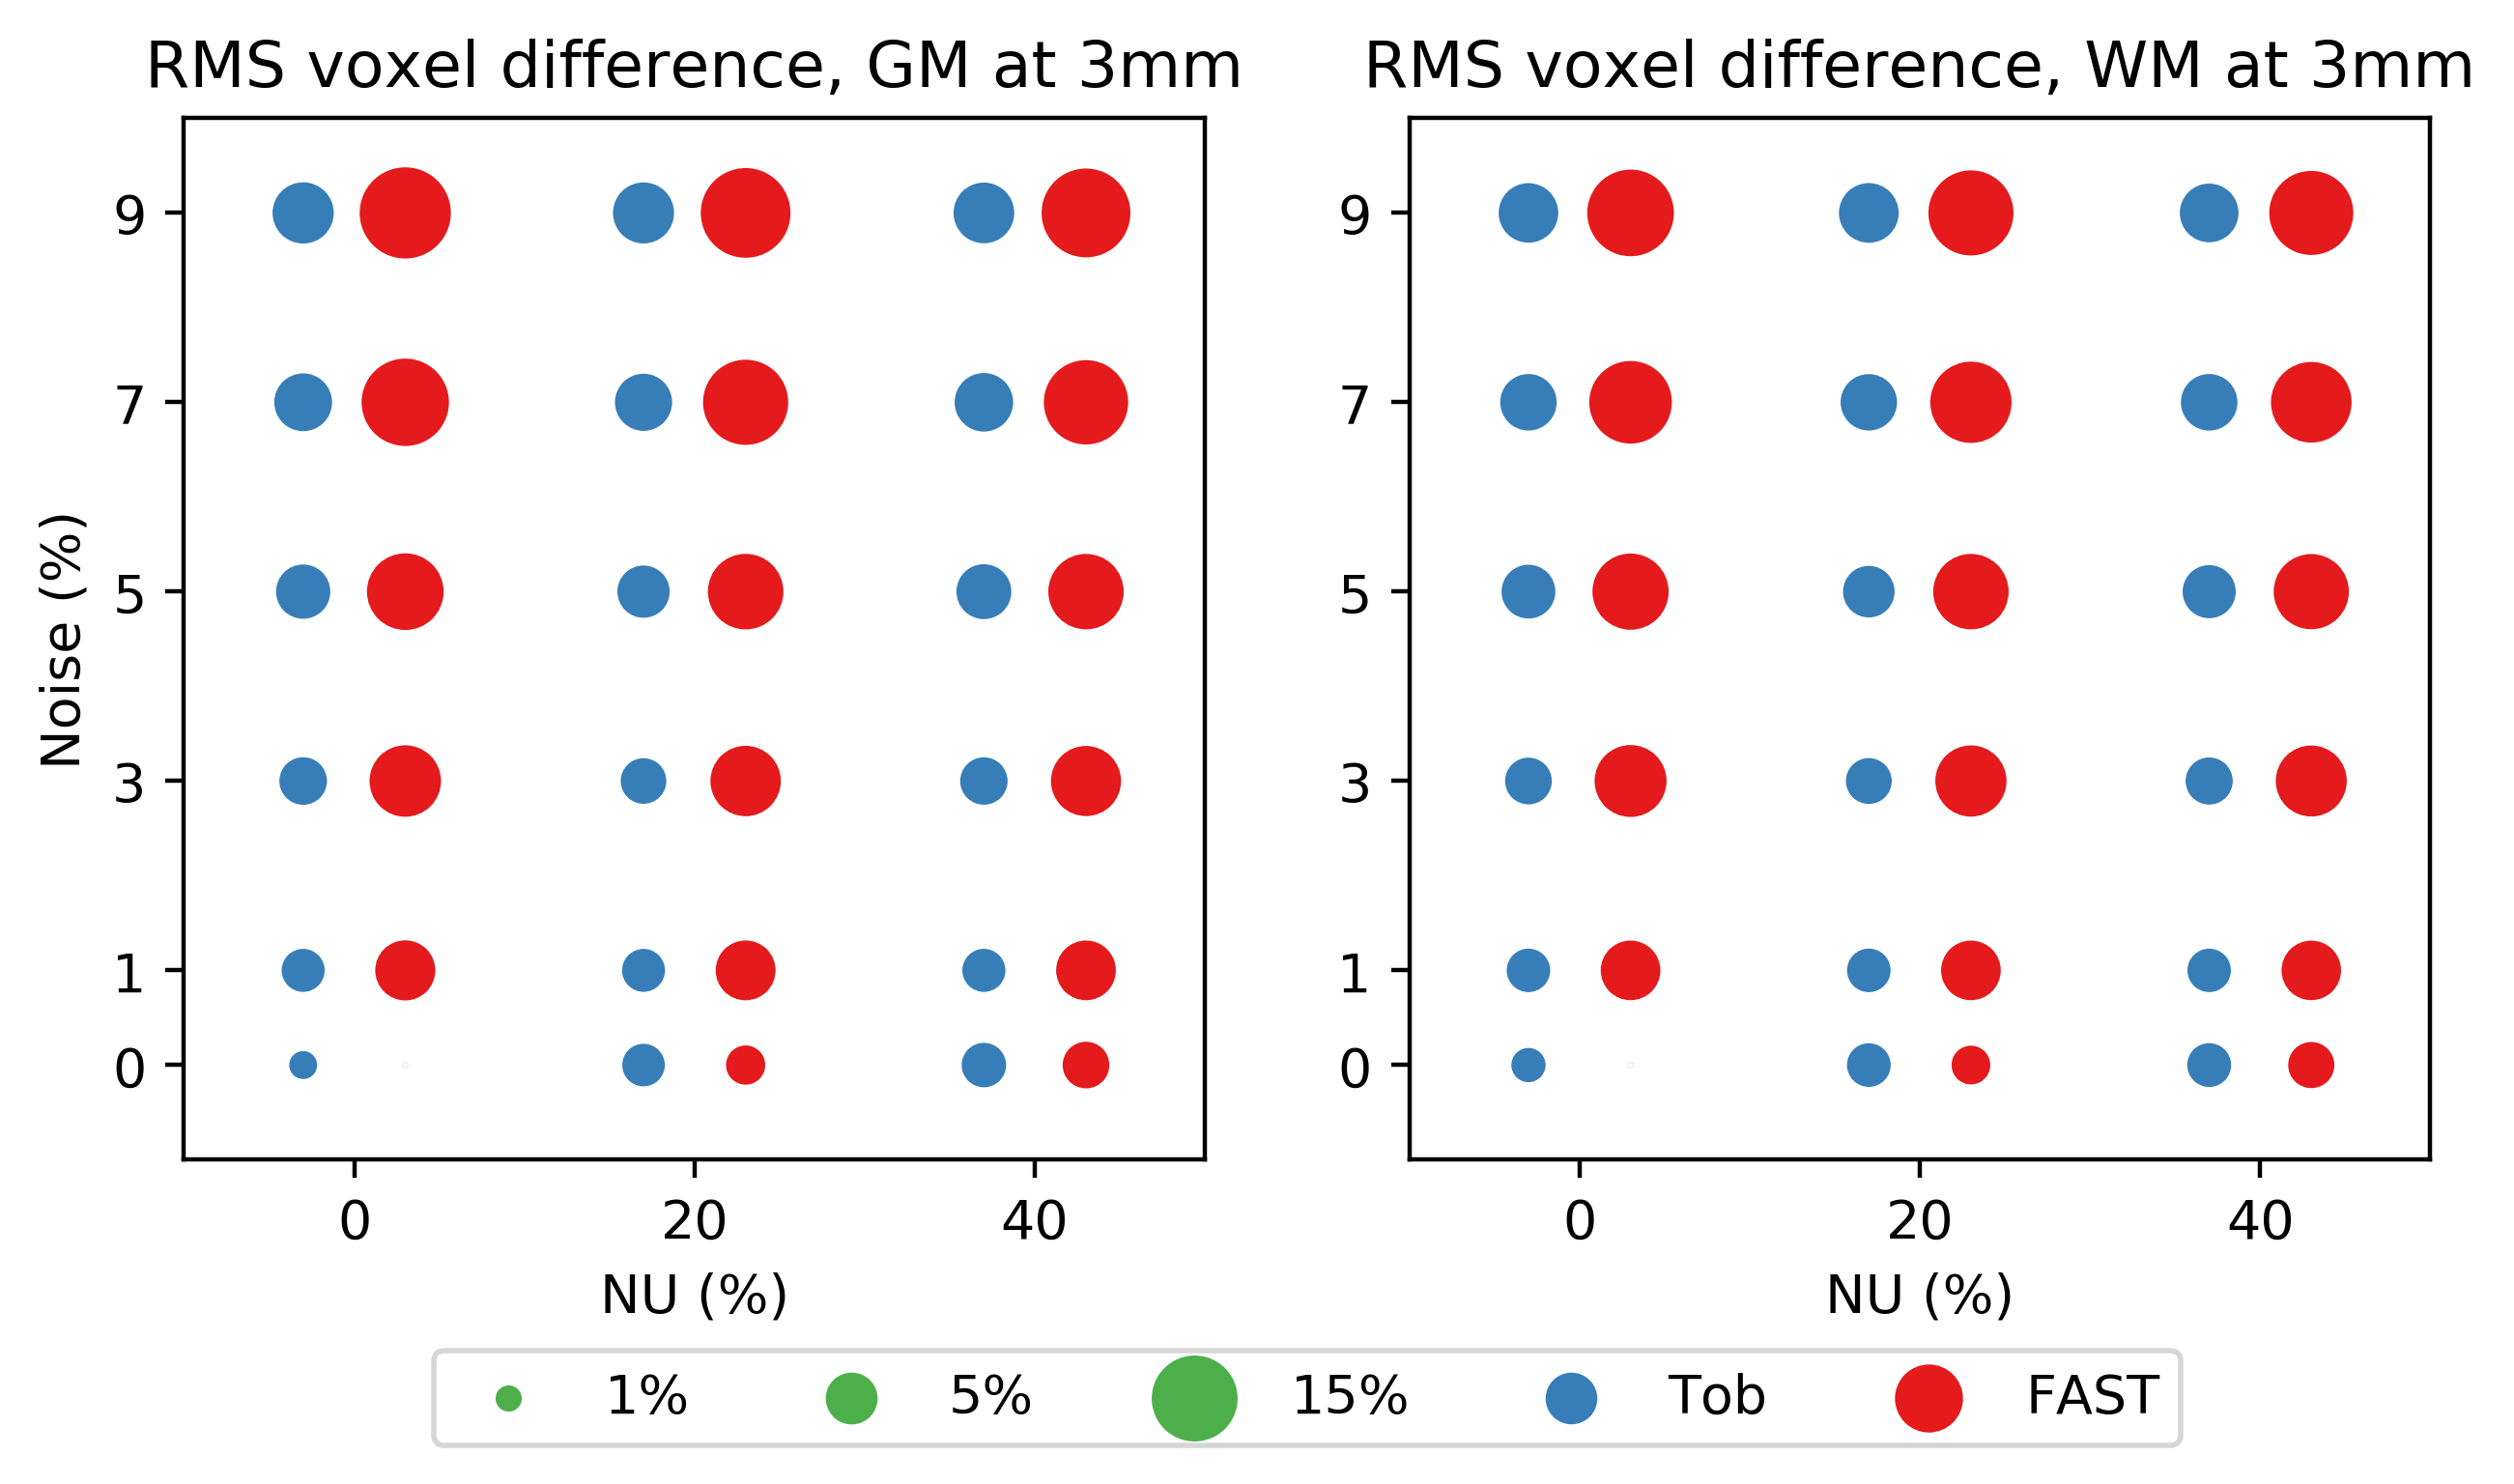
\includegraphics[width = 0.8\textwidth]{brainweb_voxel.png}
\caption{BrainWeb: RMS per-voxel differences at 3mm voxel size, referenced to each method’s 1mm 0\% noise 0\% NU results. Toblerone’s differences were smaller at almost all levels of noise and NU, as was also the case at other voxel sizes. [Results for other voxel sizes are given in the appendix, figure \ref{brainweb_voxel_supp}]}
\label{brainweb_voxel}
\end{figure}

Figure \ref{brainweb_voxel} shows the RMS per-voxel difference in PV estimates at 3mm voxel size as a function of noise and NU. Each method’s 1mm results at 0\% noise 0\% NU were used as the reference. Toblerone returned lower RMS voxel differences in both GM and WM at all levels of NU and noise except 0\% noise 0\% NU, a pattern that was repeated at other voxel sizes (given in the appendix, figure \ref{brainweb_voxel_supp}).

\subsection{HCP test-retest}

\begin{figure}[H]
\centering
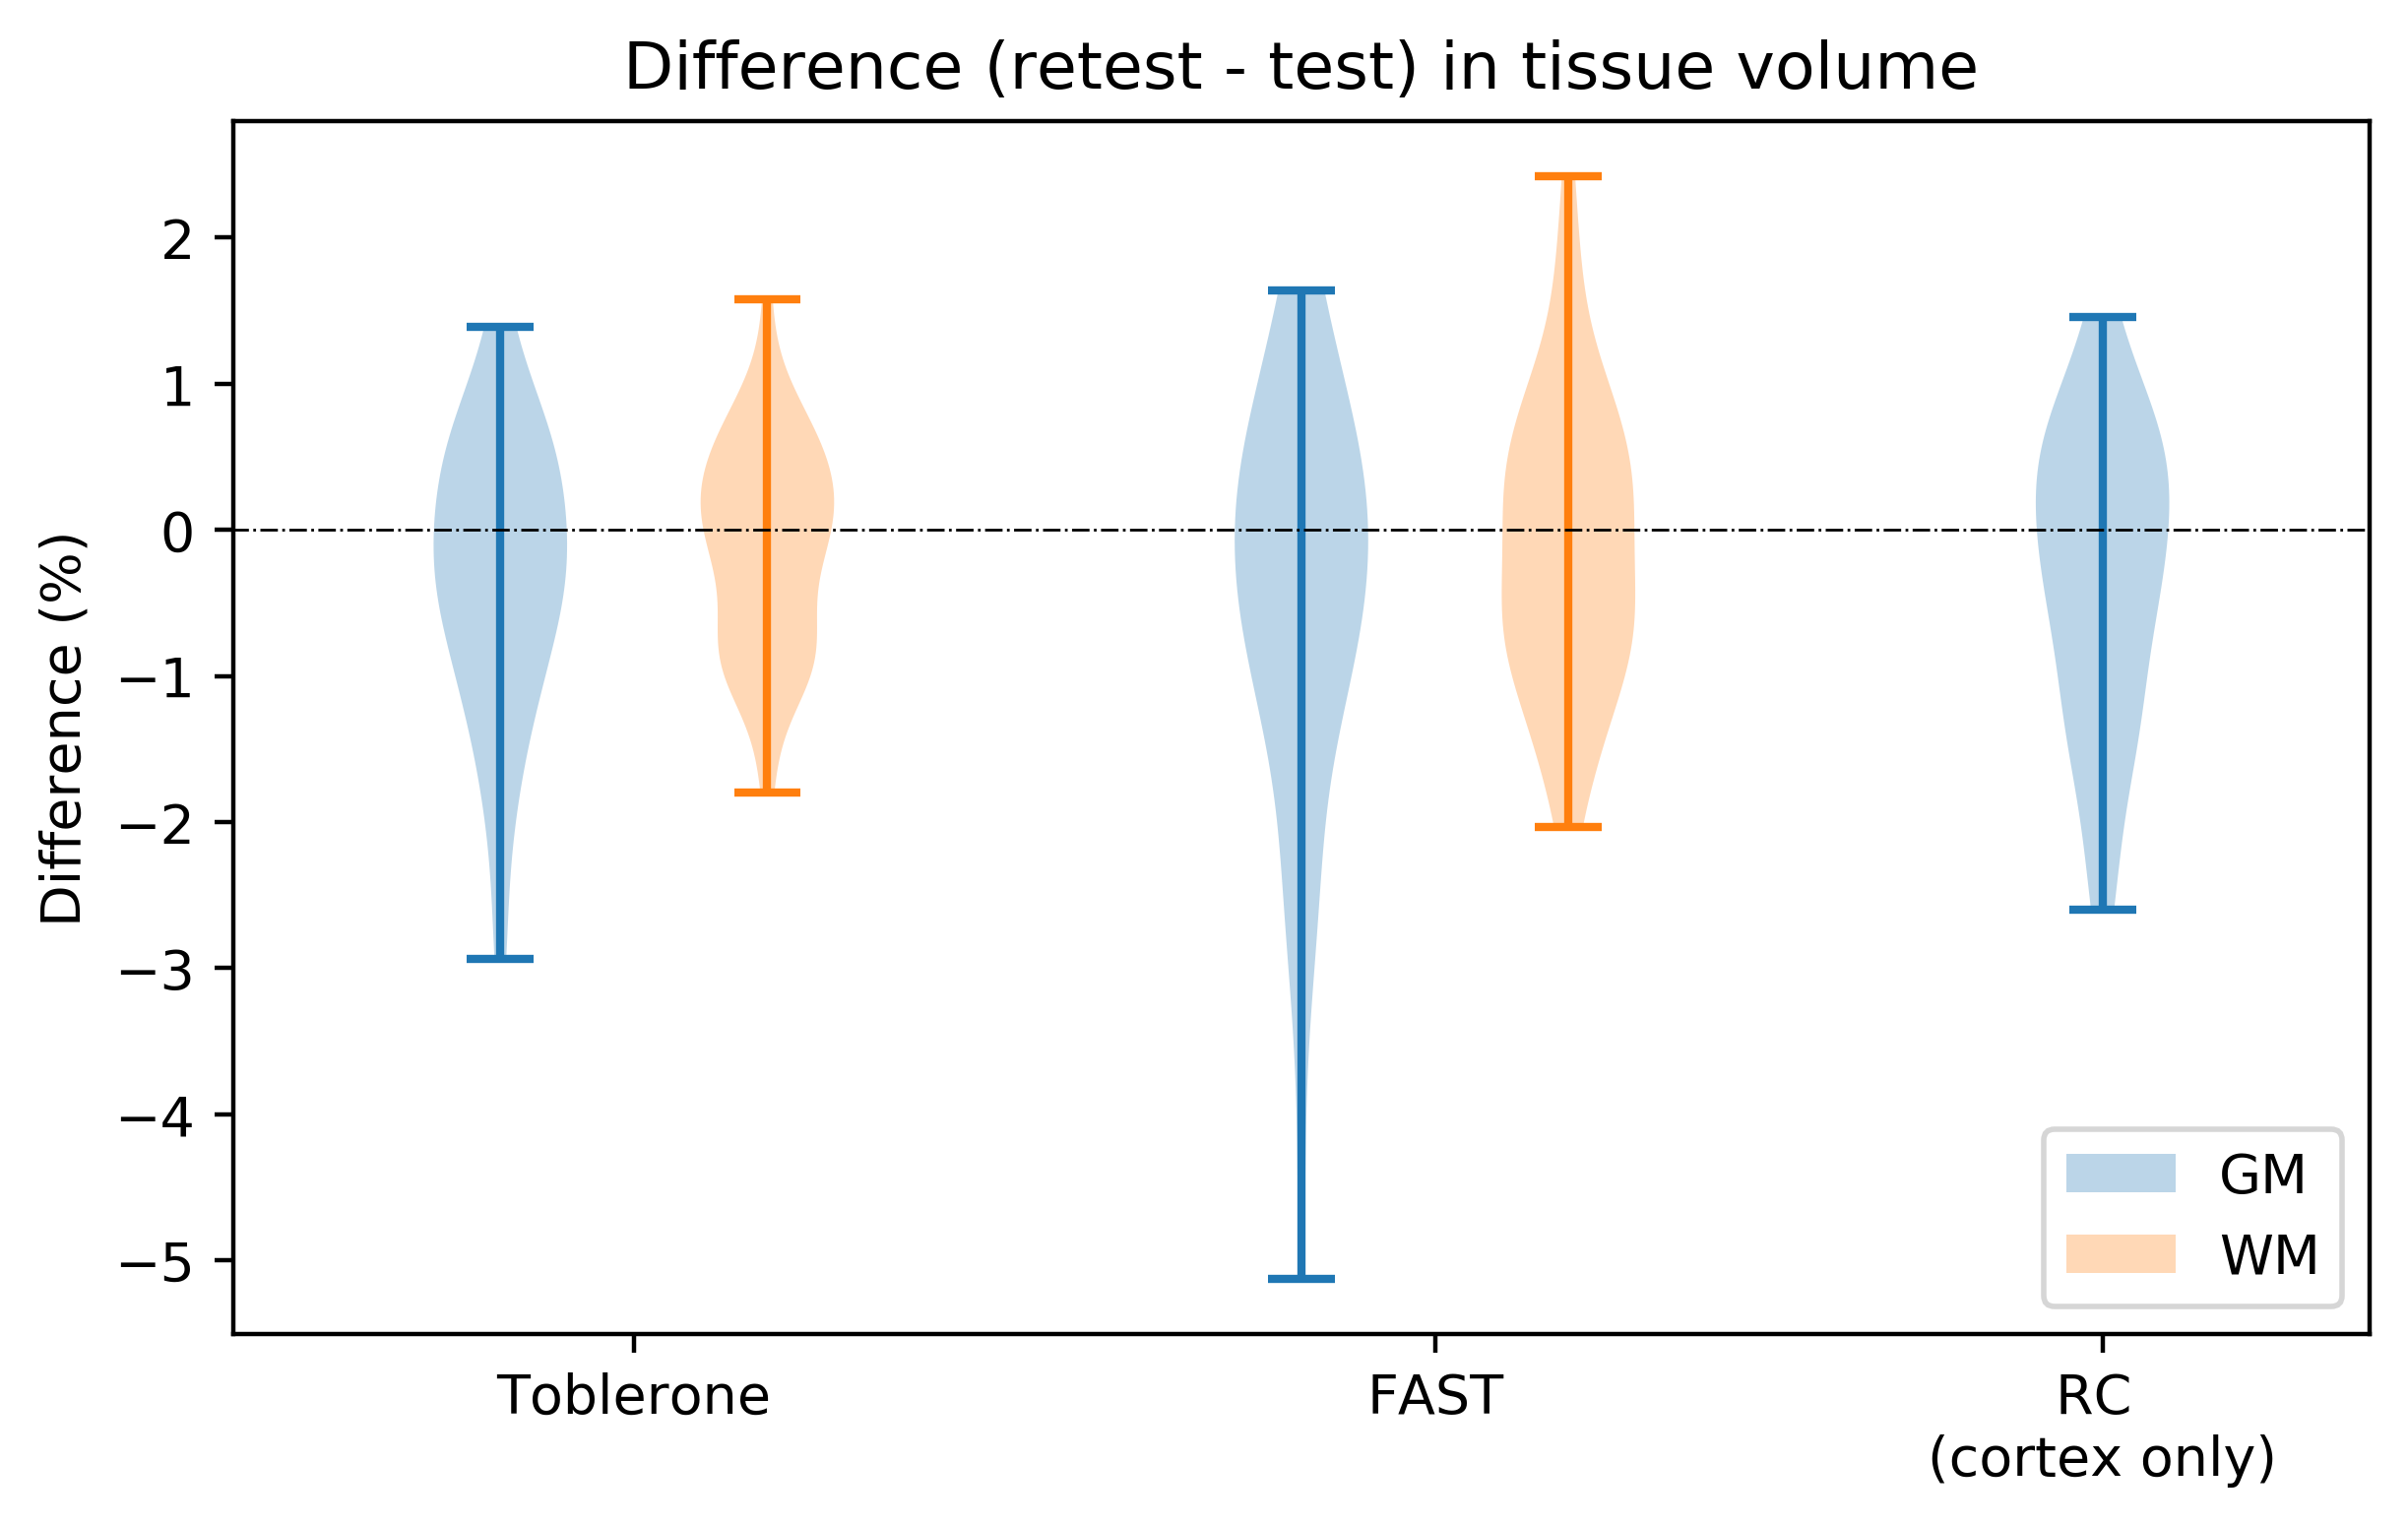
\includegraphics[width = 0.7\textwidth]{hcp_total.png}
\caption{HCP test-retest: inter-session (retest minus test) difference in total tissue volume. PVs were estimated in the native 0.7mm isotropic space of the structural images. RC’s result is for the cortex only. Both surface methods show a tighter distribution than FAST.}
\label{hcp_total}
\end{figure}

Figure \ref{hcp_total} shows violin plots of inter-session difference (retest - test) in tissue volume across the 45 subjects of the HCP dataset. PV estimates at 0.7mm isotropic voxel size were used for this analysis. RC’s GM result was for the cortex only. Both surface methods gave a tighter distribution than FAST, suggesting greater repeatability between sessions. All methods showed greater variability in GM than WM.

\begin{figure}[H]
\centering
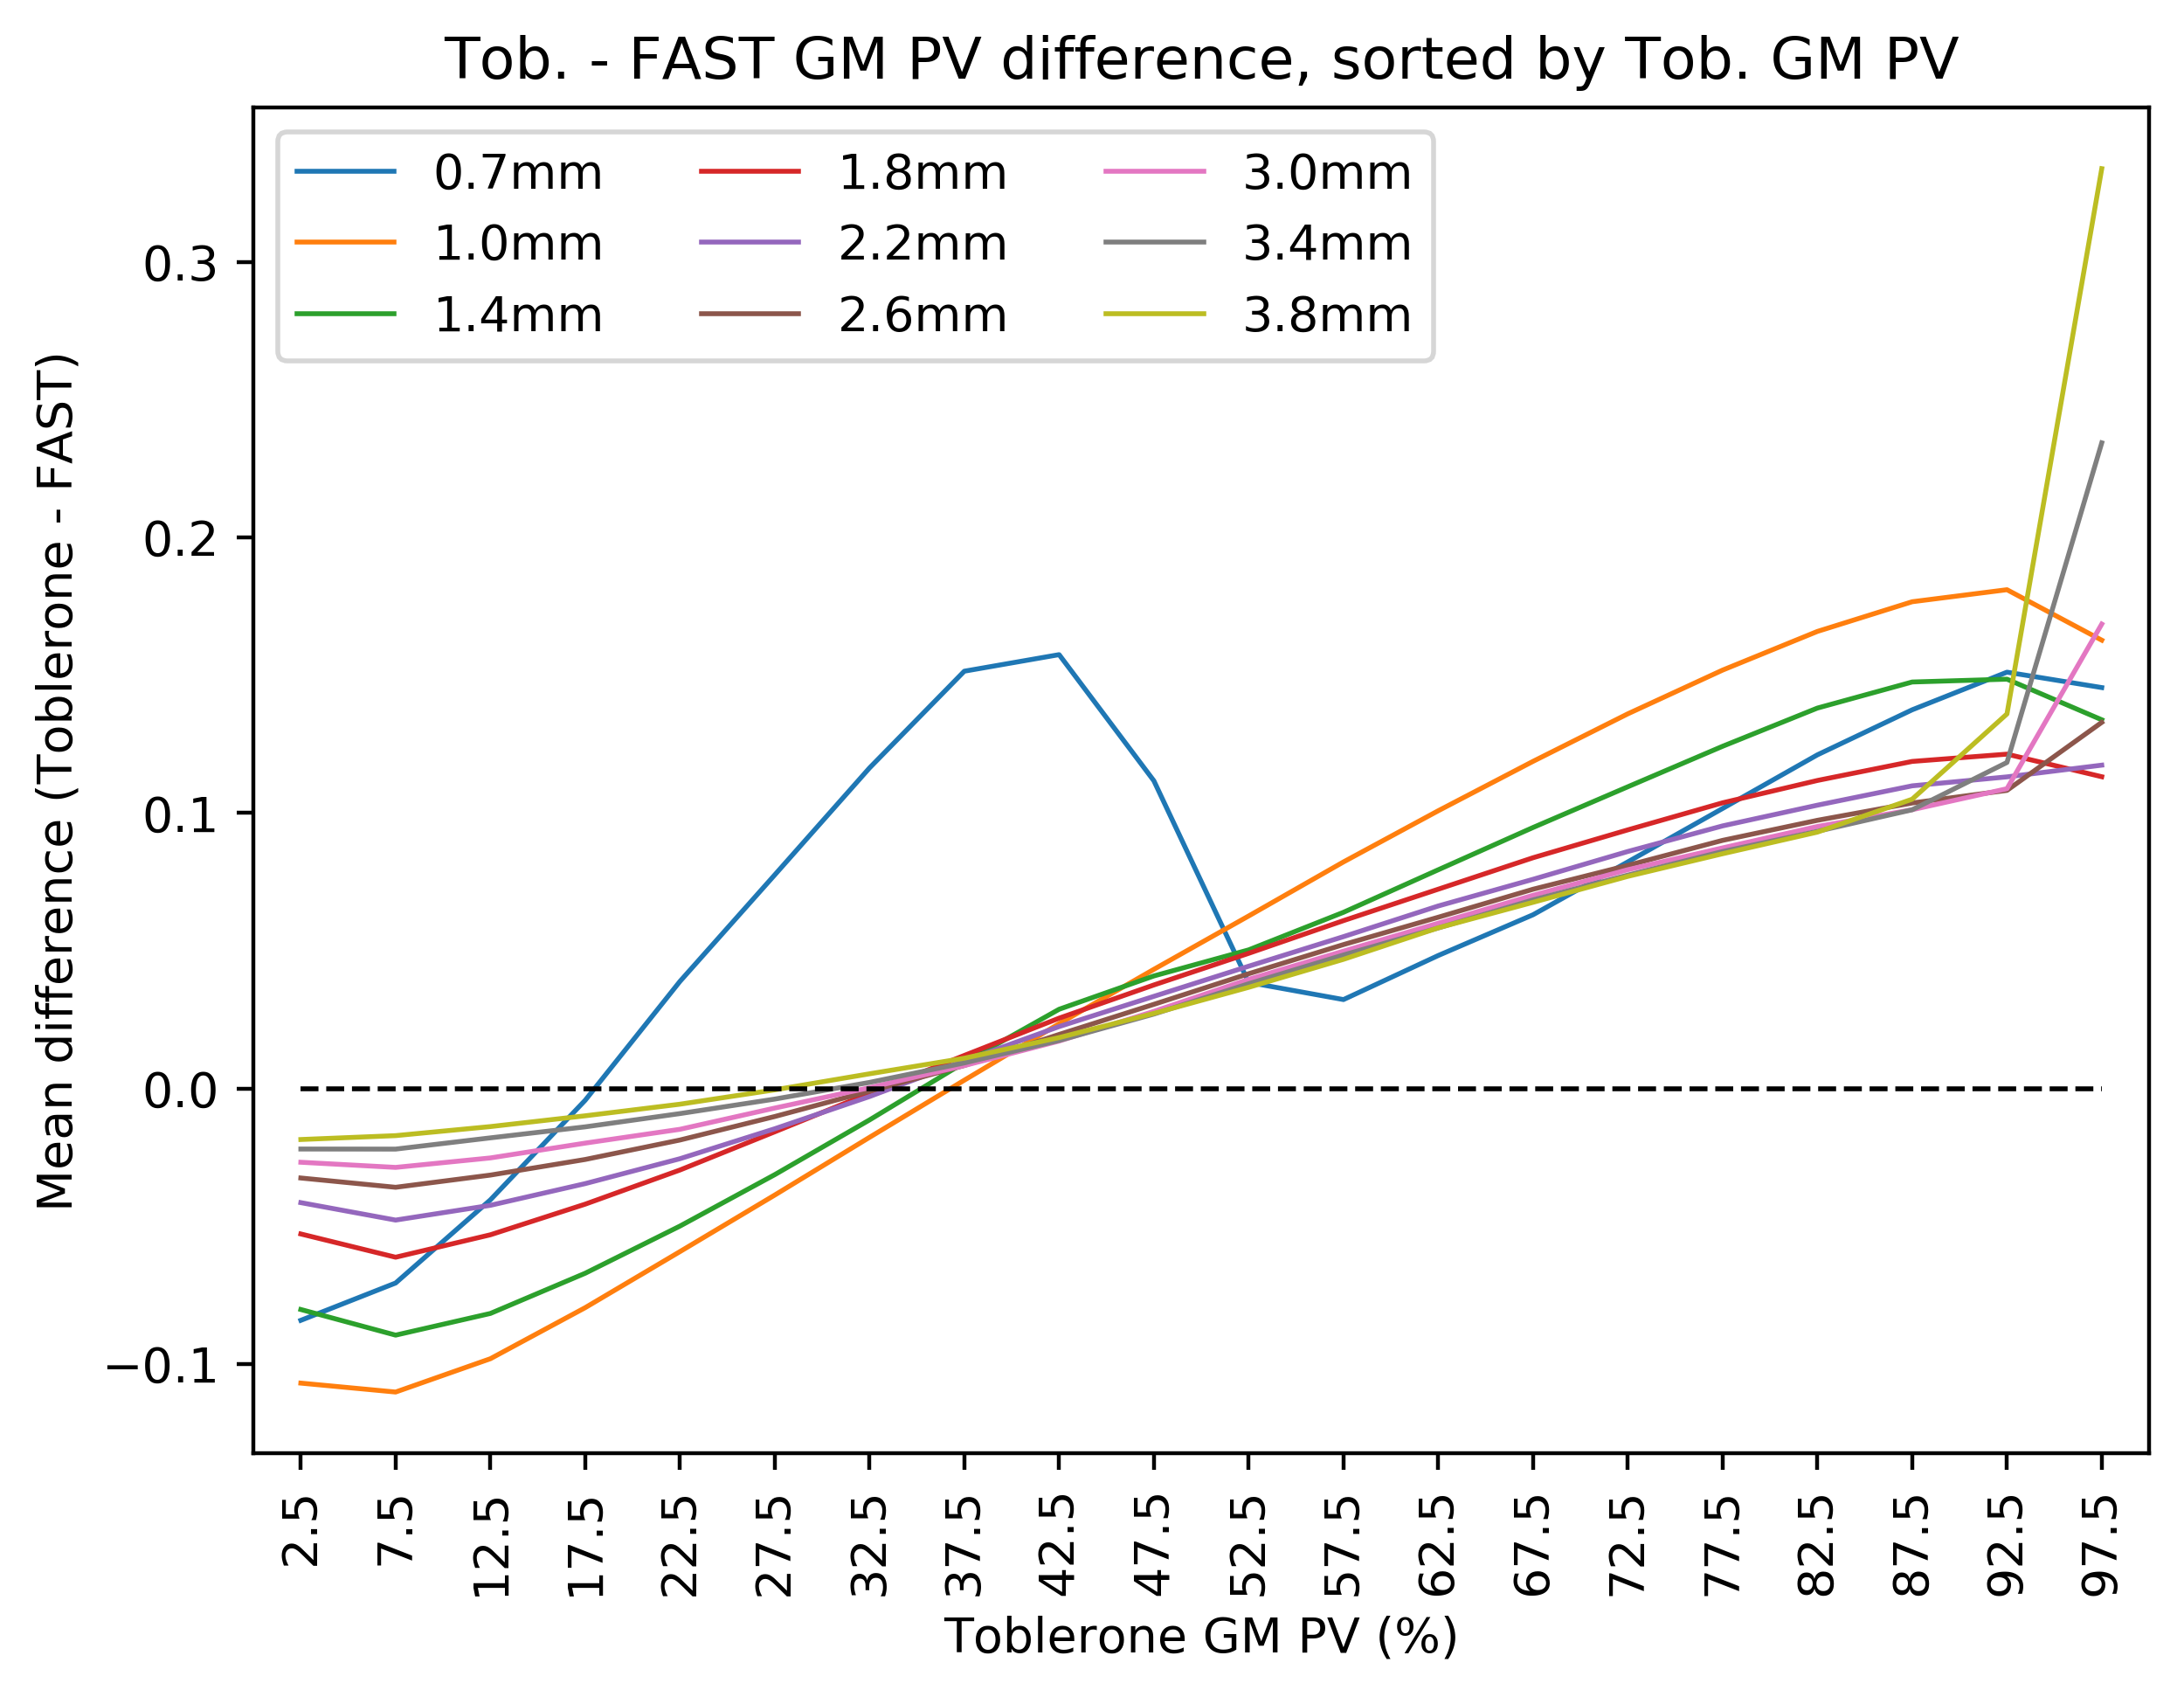
\includegraphics[width = 0.7\textwidth]{hcp_difference.png}
\caption{HCP test-retest: mean difference between Toblerone and FAST GM PVs, sorted into 5\% width bins according to Toblerone’s GM PV. As Toblerone’s GM PV estimate in a given voxel increased, FAST was more likely to assign a smaller value, and vice-versa. The strength of this relationship decreased with increasing voxel size. An inverse, but weaker, effect was seen for WM (figure \ref{hcp_difference_wm_supp} in the appendix).}
\label{hcp_difference}
\end{figure}

Figure \ref{hcp_difference} shows the mean per-voxel difference between Toblerone and FAST’s GM PV estimates as a function of Toblerone’s GM PV estimate. Excepting the 0.7mm result, the positive slope of each line shows that in voxels with a low Toblerone GM PV estimate, FAST was more likely to assign a higher value, and vice-versa at high Toblerone GM PV estimates. The strength of this relationship decreased with increasing voxel size. It should be noted that the 0.7mm result was the only one not to make use of resampling (for all others, FAST’s 0.7mm estimates were resampled onto the target voxel grid).

\subsection{\textit{In-vivo} ASL data}

\begin{figure}[H]
\centering
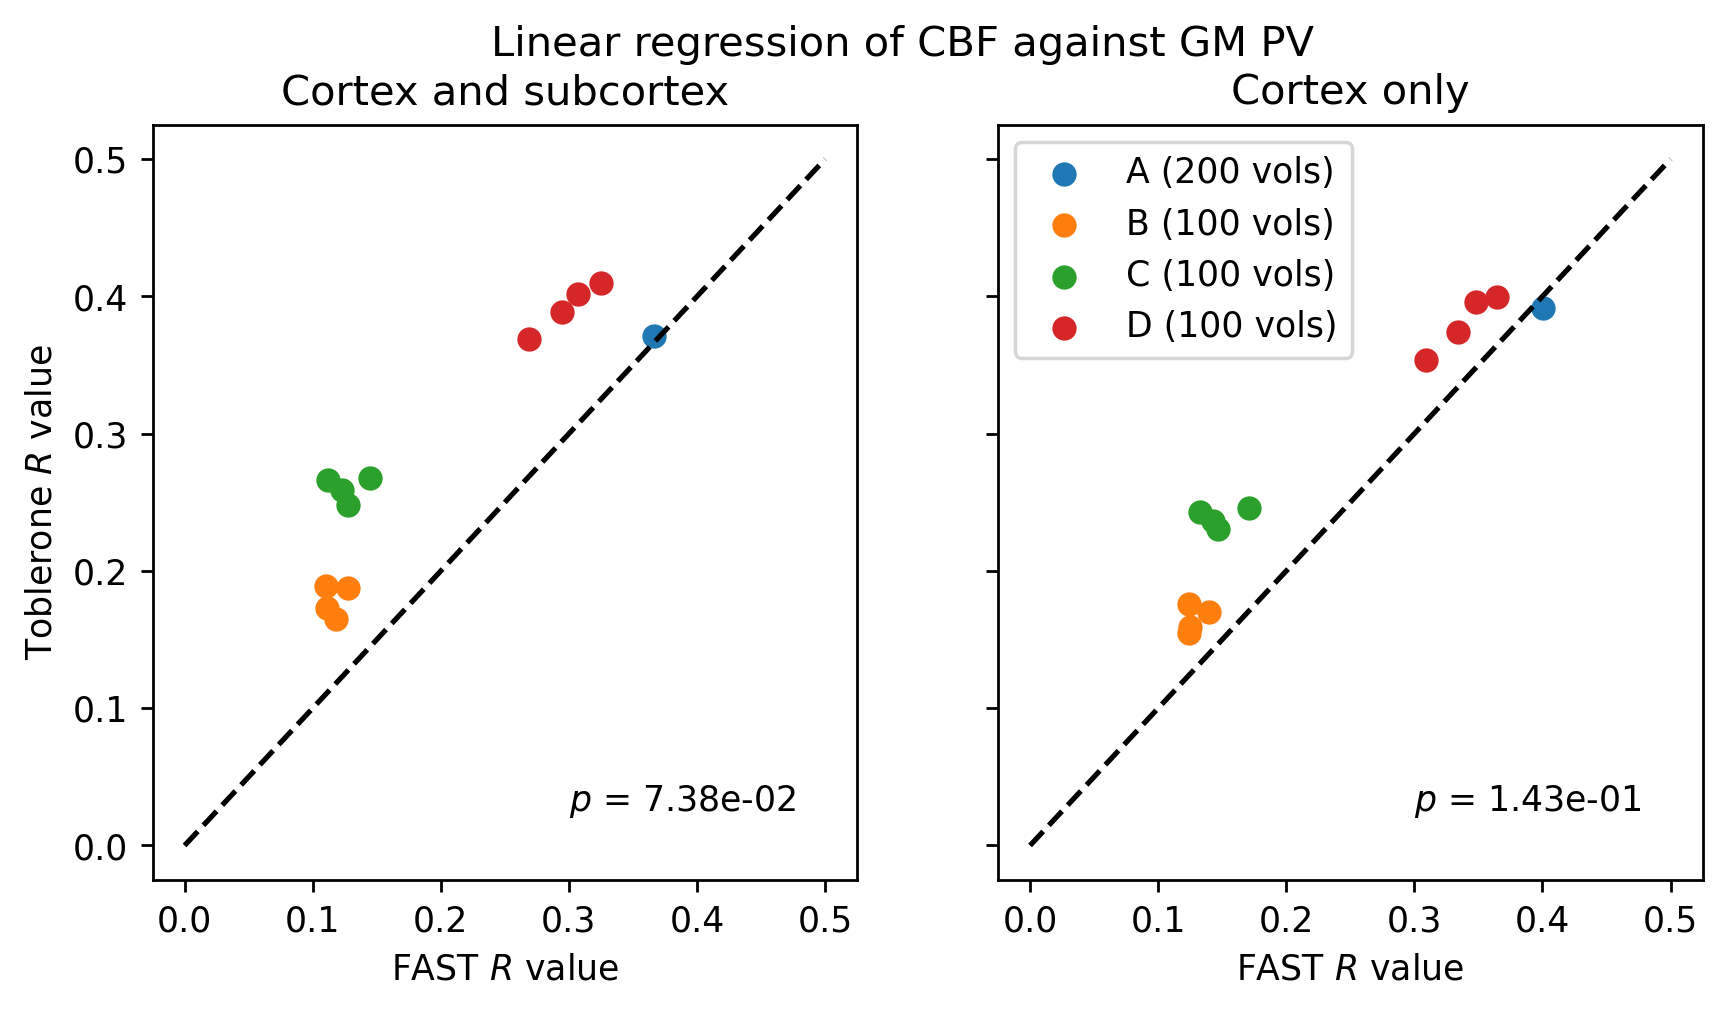
\includegraphics[width = 0.8\textwidth]{tob_vs_fast_cbf_correlation.png}
\caption{\textit{In-vivo} ASL data: correlation coefficients ($R$) of uncorrected CBF vs GM PV for FAST and Toblerone. Left: correlation against both cortical and subcortical GM. Right: correlation against cortical GM only. In almost all cases, Toblerone's estimates returned higher correlation coefficients compared to FAST, with the difference in results smaller when considering the cortex only. Significance values for a paired $t$-test comparing $R$ values are shown on each plot. }
\label{tob_vs_fast_cbf_correlation}
\end{figure}

Figure \ref{tob_vs_fast_cbf_correlation} shows correlation coefficients arising from linear regressions of uncorrected CBF against GM PV for the \textit{in-vivo} ASL data. In almost all cases, Toblerone's GM PV estimates yielded a higher $R$ value than FAST, with the difference greater when considering both the subcortex and cortex together. The variation within subjects was substantially smaller than the variation between subjects. A paired $t$-test comparison was performed by averaging $R$-values within each subject to yield four samples per method; the comparison did not meet a $p <$ 5\% significance threshold (likely due to the low number of subjects considered). 

\section{Discussion}

Results from the simulated surfaces showed that Toblerone produced estimates with a comparatively low and consistent error. Although the RC method was able to perform similarly for GM, there was a clear advantage for Toblerone in WM. Results from the BrainWeb dataset suggested that a surface-based approach (the combination of FreeSurfer/FIRST and Toblerone) was more robust to random noise and field non-uniformity than FAST’s volumetric approach. In particular, the BrainWeb results showed that the consistency of FAST’s WM estimates suffered in the presence of these real-world imperfections. Results from the HCP test-retest dataset showed that the surface-based approach provided better inter-session repeatability in estimates of total tissue volume. Finally, results from the \textit{in-vivo} ASL data demonstrated a positive trend (albeit below statistical significance) that Toblerone's PV estimates correlated better than FAST's with PVE-corrupted CBF. The difference in performance was greater when considering both the subcortex and cortex together versus the cortex only; it is known that FIRST and FAST take different views regarding the tissue composition of subcortical structures. Whilst this result does not imply that Toblerone's estimates are more `correct' than FAST's, it does suggest that a surface-based approach is better able to explain PVE-induced variation within physiological imaging data, which in turn could enable improved PVEc. 

In its native form, the RC method is unable to correctly handle voxels in which all three tissue types are present (due to the fact that it estimates only GM and then leaves the user to assign the remainder as WM or CSF based on some heuristic). The impact of this was seen in the positive relationship between per-voxel error in WM and voxel size in figure \ref{tob_sim_voxel}. Resampling can help to minimise this error: at small voxel sizes, the probability of voxels containing three tissue types is smaller and so the error is minimised, but this does not hold true at larger voxel sizes. Accordingly, as output voxel size increases, it is increasingly beneficial to obtain PV estimates by resampling those from a smaller voxel size. Set against this, however, are the aforementioned problems introduced by resampling: when the ratio of output to input voxel size is small, subvoxel effects are significant and high per-voxel errors result (as seen in figure \ref{tob_sim_voxel}). A threshold voxel value above which resampling is beneficial therefore results (at around 2mm in the figure). The exact value of this threshold would be difficult to predict in the general case (in particular, the use of aligned voxel grids in this work is both highly significant and extremely unrealistic). By contrast, Toblerone is able to produce consistent estimates in all tissue classes at arbitrary voxel sizes without the use of resampling. 

Figure \ref{hcp_difference} suggested that FAST's PV estimates were biased towards the centre of the unit interval (at least, when compared Toblerone's). For example, in a voxel that Toblerone estimated to have a low GM PV, FAST estimated a higher value, and vice-versa: in both cases, FAST's estimate was closer to the mid-point of 50\% than Toblerone's. This is possibly explained by the fact FAST uses a probability-based approach, and values in the mid-point of the interval are more likely than those at the extremes. By contrast, Toblerone's approach is purely geometric and has no knowledge of which values are more probable than others. 

It was not possible to further analyse the HCP test-retest dataset in order to establish where in the brain the differences between Toblerone’s and FAST’s estimates arise. To do so would require extensive use of non-linear registrations and resampling to transform all subjects onto a common template, and it is likely that the artefacts imposed by this process would obscure the true methodological differences of interest. Furthermore, an analysis on the BrainWeb database would be of limited use as it only represents the cortical anatomy of a single subject and would therefore ignore population variability.

\section{Conclusion}

A new method (Toblerone) has been presented for estimating PVs using surface segmentations. Unlike existing surface-based tools, it is not closely tied to any specific modality or structure and can therefore be adapted to multiple use cases (notably, providing PV estimates for the whole brain). It is able to operate at arbitrary resolutions without recourse to resampling, thereby avoiding the highly localised degradation of image quality that this process entails. Four datasets have been used for evaluation of the method. Results from simulated surfaces show consistently low errors at both the voxel and aggregate level, either matching or surpassing other surface-based methods. Results from simulated T1 images from the BrainWeb database show that a FreeSurfer/FIRST/Toblerone surface-based pipeline used as an alternative to FAST is more robust in the presence of random noise and field non-uniformity. Results from the HCP test-retest dataset of 45 subjects show that the surface-based pipeline produces a tighter distribution of inter-session tissue volumes than FAST, suggesting the surface approach has greater repeatability. Finally, a preliminary investigation using \textit{in-vivo} ASL data offers a promising hint that surface-derived estimates are better able to explain PVE-induced variation within physiological imaging data. Further analysis with a larger dataset will be required to confirm the latter result. 
